%% [PaperRefine] 施工稿。来源: paper04/paper04_CN.tex（原始稿永不修改）。复制日期: 2026-09-17。手册: PaperRefinePrompt.md。台账: paper04_CN-ledger.md。
%%
%% paper04 — 独立小论文稿(中文)
%% 模板: ACM acmart manuscript。正文已与旧 NOSR/HMACSP 叙事脱钩,仅保留版式骨架。
%% 编译: XeLaTeX(必须;见下方 ctex 说明)。
%%
\documentclass[manuscript,screen,review]{acmart}

%% ===================== 中文支持 =====================
%% scheme=plain: 只接管中文字体与断行,不改写 acmart 的章节名。
%% fontset=windows: 本机宋体/黑体; Overleaf/Linux 可改为 fontset=fandol。
\usepackage[UTF8,scheme=plain,fontset=windows]{ctex}

\usepackage{algorithm}
\usepackage{algorithmicx}
\usepackage{algpseudocode}
\usepackage{pifont}
\usepackage{makecell}
\providecommand{\checkmark}{\ding{51}}
%% B13 删去 \cmark/\xmark/\omark:定义后全稿 0 处引用(表格未采用勾叉体例)。原值见 git。
\usepackage{threeparttable}
\usepackage{tikz}
\usetikzlibrary{positioning,arrows.meta,calc,shapes,shadows}
\usepackage{xcolor}
\usepackage{amsmath}
\usepackage{bm}
\DeclareMathOperator*{\argmin}{arg\,min}
\DeclareMathOperator*{\argmax}{arg\,max}
\usepackage{multirow}
\usepackage{enumitem}
\usepackage{booktabs}
\usepackage{graphicx}
\setlength{\headheight}{20.48303pt}

%% scheme=plain 不改浮动体名称,与 paper01 中文稿对齐。
\renewcommand{\figurename}{图}
\renewcommand{\tablename}{表}
\floatname{algorithm}{算法}
\renewcommand{\proofname}{证明}

%% 机制缩写:主语是闭包,不是「修复框架」
\providecommand{\STRC}{\textsc{STRC}}
%% B13 删去 \TBD:全稿 0 处引用,待填项一律用 <待填:...> 明文标记,便于自检抓取。

%% =====================================================================
%% 主结果数字的单一来源。
%%
%% 全部由 STRC/tools/paper_numbers.py 从 STRC/experiments/expanded/*.csv 打印,
%% 数据由 `py -m tools.expand_batch` 生成(默认 5 算例 x 10 种子)。
%% 正文一律用宏,不写字面量;改数只改这里,并同步跑一遍上述两条命令核对。
%%
%% !! 2026-08-16 由 3x5=15 对扩到 5x10=50 对。旧稿所有 /15 读数一律作废。
%%
%% !! 2026-08-16(二次):E2b 由 24/50 变为 50/50。这不是换了算例,而是修掉了
%% !! 一处实现与定义的错配。释放集是一个**预约**集合,而 replay_reroute 原先
%% !! 按**工序**判定是否重路(两段中任一段进闭包就整道重规划)。于是当只有满载
%% !! 段进闭包时,同工序的空载段也被改写,而它的 task 并不在释放集里,遂被记为
%% !! 外侧漂移。26 个失败格上的 84 条漂移预约无一例外都是这种同工序空载段,
%% !! 其中 71 条(85%)在 t_now 之前就已执行完毕——改写它同时违反假设 A2。
%% !! 改为按段判定后漂移归零。据此 prop:outside 的前提 (iii) 才真正被满足,
%% !! 此前的 24/50 测的是实现缺陷,不是边集的物理覆盖度。
%% =====================================================================
\newcommand{\NInst}{5}
\newcommand{\NSeeds}{10}
\newcommand{\NPairs}{50}
%% E1/E3:两项都是满分,写成 \NPairs/\NPairs 以免手抄漏改
\newcommand{\PassMiss}{\NPairs/\NPairs}      % T_impact=0 且种子非空且原解不可行
\newcommand{\FeasRone}{0/\NPairs}            % R1 恢复可行的格数
\newcommand{\FeasRtwo}{\NPairs/\NPairs}      % R2 恢复可行的格数
\newcommand{\PassClosed}{\NPairs/\NPairs}    % E2a 结构闭合(泄漏为 0)
\newcommand{\PassInvar}{\NPairs/\NPairs}     % E2b 外侧字段逐条不变
%% E1 主批次 Cl/|R| 的逐算例极值,出处 tab:e1 表体(0.59/0.57/0.59/0.57/0.56)。
%% 此前该区间在正文三处各写一个值(0.56--0.59 / 0.54--0.57 / 0.54--0.58),即 CONFLICT-3;
%% 现统一由本宏出数。**不要**与下列同值但不同源的量混用:
%%   \ScaleCloHi(0.56) 来自规模扫描 tab:scale 的 k=4 格,是另一批次;
%%   \PubEoneFracLo/Hi 来自外部布局批次,账本独立。
\newcommand{\EoneCloLo}{0.56}
\newcommand{\EoneCloHi}{0.59}
%% 耗时(E3 批次,第 1 级改路、无扩域)
\newcommand{\MsRepairMed}{3.2}
\newcommand{\MsRepairMax}{12.8}
%% 稳定性:E5 上受 A2 约束后两臂改动比例已同区间;主对照改为 E7 的 R2 vs RA。
\newcommand{\ResFracRtwo}{50\%--66\%}
%% E5 批次:R0+ 已走固定前缀解码。降级后道改走同车续路后,18 个预算点越界均为 0。
%% 出处 expanded/e5_cross_curve.csv,`py -m tools.expand_batch --only-e5`。
\newcommand{\RzeroPastLo}{0}
%% ---------------------------------------------------------------------
%% E5 两批合读。pub_batch 直接 import expand_batch 的 _run_e5,
%% t_now_frac=0.35、预算 {0.2,1,2}s、pop=40、hot=True 逐项同一,故可合池;
%% 两批只差布局出处(自建 / 外部转录),这正是合池的意义。
%% 出处 expanded/e5_cross_curve.csv + pub_layouts/e5_cross_curve.csv,
%% 复算脚本 tools/_p17_e5_stats.py。
\newcommand{\EfiveInst}{4}          % congested_8x4x4, example_3x3x2, LyuL2_4m, LyuL6_8m
\newcommand{\EfiveCells}{12}        % 独立算例--随机种子格
\newcommand{\EfivePts}{36}          % 预算点总数 = 12 格 x 3 档
\newcommand{\EfiveWLT}{35/1/0}      % 逐预算点 R0+ 胜/持平/负
\newcommand{\EfiveWinMin}{11}       % 最小预算档上 R0+ 严格更优的格数
\newcommand{\EfiveTieMin}{1}        % 同,持平的格数(LyuL6_8m, 种子 2024)
%% ---------------------------------------------------------------------
%% 离散度口径(P17)。均值表/图一律配一个四分位距,免得只读到均值。
%% 出处同上脚本;E1 为 expanded/e1_miss.csv 逐算例 10 种子。
\newcommand{\EoneFracIqrLo}{0.024}  % 逐算例 Cl/|R| 的 IQR 最小值
\newcommand{\EoneFracIqrHi}{0.049}  % 同,最大值
\newcommand{\EoneFracMed}{0.571}    % 50 对合池中位
%% 合池 IQR 实测 0.0372,与 §5 的 Hodges--Lehmann 估计 0.037 同值\emph{不同源};
%% 为免两个不相干的量在正文里撞成一个读数,此处不出宏、图注也不报该值,
%% 只报逐算例 IQR 区间与合池极差,已足够说明离散度。
\newcommand{\EoneFracMin}{0.500}    % 50 对合池极差下端
\newcommand{\EoneFracMax}{0.655}    % 同,上端
%% phi 扫描(tab:scale / fig:scale):耗时极差与 Cmax 逐档 IQR
\newcommand{\ScaleMsMin}{2.2}       % 全扫描 strc_wall_ms 极差下端
\newcommand{\ScaleMsMax}{23.8}      % 同,上端
\newcommand{\ScaleCmaxIqrLo}{8}     % 逐档 R0+ Cmax 的 IQR 最小值
\newcommand{\ScaleCmaxIqrHi}{76}    % 同,最大值
%% 规模扫描的加速比区间(跨两算例的逐格极值)
\newcommand{\SpeedLo}{87}
\newcommand{\SpeedHi}{3051}
%% E6:A 类上闭包严格大于工序依赖图释放集的格数(其余格两者相等,不是包含失败)
\newcommand{\StrictlyLarger}{87/100}
%% E6:闭包占 t_now 之后活预约的比例(走廊阻断)。这个数偏大,
%% 是「不作最小性主张」那条注记的实测依据,不要美化。
\newcommand{\ClosureAliveFrac}{92\%}
%% =====================================================================
%% 外部来源布局批次(STRC/experiments/pub_layouts/)。**独立账本**,不并入上面的
%% \NPairs 对——把它混进主批次会让全部 /\NPairs 读数改口径。两批算例逐参数同口径,
%% 只差布局来源。数出处:py -m tools.pub_batch 后 py -m tools.paper_numbers。
%% 边权是本文补齐的等权值,故这批数**不可**与 Lyu 或 van Os 的参照值比较。
%% =====================================================================
\newcommand{\NPubInst}{5}
\newcommand{\NPubPairs}{50}
\newcommand{\PubPassMiss}{\NPubPairs/\NPubPairs}
\newcommand{\PubFeasRone}{0/\NPubPairs}
\newcommand{\PubFeasRtwo}{\NPubPairs/\NPubPairs}
\newcommand{\PubPassClosed}{\NPubPairs/\NPubPairs}
\newcommand{\PubPassInvar}{\NPubPairs/\NPubPairs}
\newcommand{\PubEoneFracLo}{0.438}
\newcommand{\PubEoneFracHi}{0.547}
%% E4 同参数对照。**这里的口径要格外小心,曾写错过一次。**
%% \NPubInst 个外部算例只落在 \NPubNets 张不同路网上(4x4 去一条边:LyuL2/L3;
%% 5x5 去两条边:LyuL4/L5/L6),差别在机器台数与落位。于是:
%%   \PubCloSpread 这个极差的两个端点(\PubCloHi=LyuL2 4 机、\PubCloLo=LyuL3 5 机)
%%   **共享同一张路网**,所以它测的是机器落位,**不是**路网几何。
%%   不要再写成"闭包占比随布局显著变化"——数据不支持这句。
%% 正确的用法是:同一路网上换落位即得 \PubCloSpread,而 LU 最小割与漏斗占比全程恒定
%% (两张路网都把装卸站放在网格角点,四邻接下角点恰两条出边),故静态割被干净否证。
%% 注意别把这句写成"公开布局一律放在角点":工具集另附的 Liu 那族放在网格边中点(出度 3),
%% 只是因允许对角移动而未收入。准确的说法是该指标只取到极少数由摆位决定的离散值。
\newcommand{\NPubNets}{2}
\newcommand{\PubCloLo}{0.305}
\newcommand{\PubCloHi}{0.512}
\newcommand{\PubCloSpread}{0.207}
\newcommand{\PubCloSpreadBig}{0.075}
\newcommand{\SelfCloLo}{0.446}
\newcommand{\SelfCloHi}{0.497}
\newcommand{\SelfCloSpread}{0.051}
\newcommand{\PubEfiveNoCross}{17/18}
%% =====================================================================
%% 便宜对照臂(E7)与算例规模扫描(E8)。两批共用同一组臂定义:
%%   RS  全局右移。不改路径/指派/序,把未完成的一切统一后推到阻断窗之后。
%%       冻结判据与 R2 相同(t_end <= t_now 不可动),故按 A2 可采纳。
%%   RD  原染色体重解码。保持机器指派与扫描序,走与 R0+ 同一套固定前缀解码。
%%       降级后道改走同车续路后,A2 越界为 \RedecodeBad。
%%   RA  不划边界:释放 t_now 之后的全部预约,再走与 R2 完全相同的改路重放。
%%       它与 R2 共用引擎、共用冻结判据,唯一差别是释放集取了平凡上界,
%%       故 R2--RA 之差可全部归因于闭包这个对象本身。
%% 出处:STRC/experiments/cheap_baselines.csv (py -m tools.cheap_baselines)
%%      STRC/experiments/scale_curve.csv     (py -m tools.scale_curve)
%% 协议与 E1--E3 一致(繁忙走廊单窗阻断、t_now=0.35 Cmax、R2 不开扩域),
%% 故 tab:cheap 可与 tab:e3 并读;但**不可**与 tab:e5 并读——那批只有两个算例。
%% =====================================================================
\newcommand{\MsShift}{1.42}          % RS 耗时中位/ms(\NPairs 对)
\newcommand{\MsRedecode}{4.16}       % RD 耗时中位/ms(同上)
\newcommand{\MsAllFuture}{2.76}      % RA 耗时中位/ms(同上)
\newcommand{\MsCheapRtwo}{2.74}      % 同批 R2 的耗时中位,供四臂同口径比较
\newcommand{\RedecodeRatio}{1.5}     % MsRedecode / MsCheapRtwo
\newcommand{\ShiftBad}{0/\NPairs}    % RS 改写已完成预约的格数
\newcommand{\RedecodeBad}{0/\NPairs}
\newcommand{\WinVsShift}{27/16/7}    % R2 对 RS 的 Cmax 赢/平/输
\newcommand{\WinVsRedecode}{14/14/22}
\newcommand{\WinVsAllFuture}{4/46/0}
\newcommand{\ResFracCheapRtwo}{0.540}
\newcommand{\ResFracShift}{0.627}
\newcommand{\ResFracRedecode}{0.618}
\newcommand{\ResFracAllFuture}{0.604}
%% R2 对 RA 的逐格稳定性对比(改动比例;两臂都可行的 \NPairs 格全部纳入)。
\newcommand{\RAStabWTL}{31/18/1}     % R2 更稳/持平/更差
\newcommand{\RAStabP}{8.8\times10^{-7}}  % Wilcoxon 符号秩,双侧
\newcommand{\RAStabMean}{0.064}      % 改动比例平均降幅
%% 下面两个是剔除 6 个「两法恒等」格(R2 释放集 = 全部未结束占用)后的同一读数,
%% 由 STRC/tools/audit_checks.py 自 cheap_baselines.csv 直算;剔除使降幅变大。
\newcommand{\RAStabWTLNet}{31/12/1} % 剔除恒等格后的 R2 更稳/持平/更差(n=44)
\newcommand{\RAStabMeanNet}{0.073}  % 同,平均降幅
\newcommand{\RAStabMed}{0.029}       % 同,中位降幅
\newcommand{\RACmaxRatio}{0.999}     % Cmax 比 R2/RA 均值
\newcommand{\RACmaxLo}{0.970}        % 同,最小值(R2 最占优的那格)
\newcommand{\ClosureShareLo}{0.80}   % 闭包/全部未来预约:最小值
\newcommand{\ClosureShareMean}{0.92} % 同,均值(与 \ClosureAliveFrac 同源)
%% 算例规模梯子:工件 2k、机器 k、车 k,k=4..10;拥堵档、H、F、Tt/Tp 与两处割集同口径,
%% 只有规模变(生成器 clbs/tools/gen_instances.py 的标定见其文档字符串)。
\newcommand{\ScaleKs}{7}
\newcommand{\ScalePairs}{70}
\newcommand{\ScaleJobsHi}{20}
\newcommand{\ScaleMachHi}{10}
\newcommand{\ScaleCloLo}{0.48}       % 闭包占全表比例:k=10
\newcommand{\ScaleCloHi}{0.56}       % 同,k=4
%% 下面三个与上面两个是同一批数据的两种分母,由 tools/audit_checks.py 自 scale_curve.csv
%% 的 n_res / n_live / closure 三列直算(不是反推)。Cl/|R| 的可达上界是 |R^o|/|R|,
%% 故回答「占比会不会涨到接近 1」必须用 Cl/|R^o| 这一口径。
\newcommand{\ScaleAliveShare}{0.61}  % 均 |R^o|/|R|,七档均值 0.611
\newcommand{\ScaleCloAliveLo}{0.78}  % 闭包占尚未结束占用之比,档均值最低:k=10 的 0.782
\newcommand{\ScaleCloAliveHi}{0.91}  % 同,最高:k=4 的 0.905
\newcommand{\ScaleMsHi}{10.4}        % R2 耗时中位:k=10
\newcommand{\ScaleRatioLo}{1.5}      % RD/R2 耗时比:k=4
\newcommand{\ScaleRatioHi}{3.3}      % 同,k=10
\newcommand{\ScaleFeasFirst}{69/\ScalePairs}   % 第 1 级改路即可行的格数
\newcommand{\ScaleFeasAll}{\ScalePairs/\ScalePairs}
%% E7 事后规则:释放占比 vs 稳定性降幅。阈值在 cheap_baselines.csv 本样本上选定,
%% 不作外推定理。出处:py -m tools.paper_numbers(worth_section)/fig_strc_worth_CN.py
\newcommand{\WorthThresh}{0.93}
\newcommand{\WorthLowN}{27}
\newcommand{\WorthLowMean}{0.094}
\newcommand{\WorthHighN}{23}
\newcommand{\WorthHighMean}{0.029}
\newcommand{\WorthVanish}{0.97}
%% 边集差分试探。出处:STRC/experiments/edge_probe.csv (py -m tools.edge_probe --full)
\newcommand{\ProbeLeakPairs}{0/50}
\newcommand{\ProbeLeaks}{0}
%% E6 修复维(第 1 级、不开扩域)。出处:expanded/e6_types.csv 的 R2_feasible 列
\newcommand{\FeasESixBlock}{\NPairs/\NPairs}
\newcommand{\FeasSlow}{\NPairs/\NPairs}
\newcommand{\FeasESixAgv}{\NPairs/\NPairs}
\newcommand{\FeasESixRa}{\NPairs/\NPairs}
%% 非均匀边权 E1/E3。出处:STRC/experiments/weight_sweep.csv (py -m tools.weight_sweep)
\newcommand{\WeightLogRtwo}{\NPairs/\NPairs}
\newcommand{\WeightLuRtwo}{\NPairs/\NPairs}
\newcommand{\WeightSplitRtwo}{49/\NPairs}

\usepackage{amsthm}
\newtheorem{assumption}{假设}
\newtheorem{definition}{定义}
\newtheorem{problem}{问题}
\newtheorem{remark}{注}
\newtheorem{prop}{命题}
\newtheorem{lem}{引理}

\AtBeginDocument{%
  \providecommand\BibTeX{{%
    Bib\TeX}}}

\setcopyright{acmlicensed}
\copyrightyear{2026}
\acmYear{2026}
\acmDOI{XXXXXXX.XXXXXXX}

%%\acmSubmissionID{123-A56-BU3}

\begin{document}

%% =====================================================================
%% 标题:独立小论文用「工序依赖图覆盖不到」钩子;大论文章题另用「闭包上的有界修复」
%% B11 定名:题名与正文统一用「工序依赖图」(CONFLICT-4);删「级联」二字——该词全稿
%% 仅题目一处,正文与贡献、结论一律作「损坏」,删后逐字一致且全标题回到 29 字(≤30)
%% =====================================================================
\title[工序依赖图覆盖不到的损坏]{工序依赖图覆盖不到的损坏:无冲突柔性作业车间的时空预约闭包}

\author{Qi Yu}
\email{230240012@seu.edu.cn}
\orcid{0009-0008-7843-6345}
\affiliation{%
	\department{School of Cyber Science and Engineering}
	\department{Key Laboratory of Computer Network and Information Integration}
	\institution{Southeast University}
	\city{Nanjing}
	\state{Jiangsu}
	\country{PR China}
}

\author{Wei Li}
\orcid{0009-0001-0949-329X}
\email{xchlw@seu.edu.cn}
\authornote{corresponding author}
\affiliation{%
	\department{School of Computer Science and Engineering}
	\department{Key Laboratory of Computer Network and Information Integration}
	\institution{Southeast University}
	\city{Nanjing}
	\state{Jiangsu}
	\country{PR China}
}

\renewcommand{\shortauthors}{Yu and Li}

%% =====================================================================
%% 摘要
%% 骨架:背景缺口 → 主张(边界在预约图) → 对象 STRC → 用法(有界修复) →
%%       与全局重解分工(响应时间一侧) → 实验钩子(不把创新挂在「又一个修复算法」上)
%% =====================================================================
\begin{abstract}
在同时用工序依赖刻画加工先后、又用时间窗预约记录走廊占用的柔性作业车间调度中,
扰动后划定重调度范围的现成做法仍是先找出受影响工序、再连同其后续一并重排。
但走廊在某段时窗内不可通行或通行变慢时,没有任何工序因此无法执行,
该做法给出空范围、判为无需重调度;而落在受扰时段内的走廊占用已经失效,原排程不可行,
等待还会沿让行关系传给后续车辆。缺口不在检测,而在以工序为节点的依赖图
不含走廊占用之间的让行关系。

本文把重调度范围定义在走廊占用及其依赖关系上,给出时空预约闭包(\STRC),
正文亦称预约影响集:以占用时段与扰动时窗重叠的走廊预约为起点,沿同走廊让行、
同一车辆的后续占用、同一工件与同一机器下一道工序的占用这四类边取传递闭包;
集内占用允许改写,集外沿用原计划。依赖边一经给定,一条占用是否属于该集即唯一确定,
不随改路算法的实现而变。恢复分两级:先在集内为原车改路,仍不可行时再按既定顺序
扩大允许改写的范围。

在 \NInst\ 算例 \(\times\) \NSeeds\ 个随机种子共 \NPairs\ 对上,走廊阻断时按工序依赖图
划出的范围 \PassMiss\ 为空而原排程确已不可行;同一套改路程序只换划界对象,
恢复可行率由 \FeasRone\ 变为 \FeasRtwo;集内没有指向集外的依赖边、集外占用的走廊、
时段与车辆逐条不变,两项各 \PassClosed\ 与 \PassInvar。把允许改写的集合换成
「决策时刻之后尚未结束的全部占用」、其余一切不变时,耗时与完工时间几乎不动,
改写比例却由 \ResFracCheapRtwo\ 升到 \ResFracAllFuture(逐格 \RAStabWTL,
Wilcoxon 符号秩双侧 \(p=\RAStabP\))。相对不改写已结束占用的热启动全局重调度,
有界修复耗时低两到三个数量级,但完工时间在全部预算档上更差,
且放宽预算不出现反超。

本文主张的是划界对象,不是一种新的修复策略:集内改路、集外保持、失败后扩大范围
都已见于既有工作。影响集不作最小性声称,它覆盖决策时刻尚未结束的走廊占用约
\ClosureAliveFrac;少改写这一项收益取决于它比该平凡上界少纳入多少,
在两者接近时趋于消失。完工时间上,有界修复不能替代全局重调度。
\end{abstract}

\keywords{柔性作业车间调度, AGV 无冲突路由, 时空预约表, 时空预约闭包, 走廊阻断}

%% CCS。投 ACM 时须用官方工具重生成 CCSXML 块;此处先给 \ccsdesc 以消除
%% acmart 对超过两页稿件的 "no CCS concepts" 警告。非 ACM 场合整段可删。
\ccsdesc[500]{Theory of computation~Scheduling algorithms}
\ccsdesc[300]{Applied computing~Industry and manufacturing}
\ccsdesc[300]{Computing methodologies~Planning and scheduling}

\maketitle

%% =====================================================================
\section{引言}
\label{sec:introduction}
%% =====================================================================

\subsection{背景与动机}

考虑运输的柔性作业车间调度长期建立在一个便利假设之上：工件在两台机器之间的移动时间是一个常数，可从按位置对索引的矩阵中读出。
该假设默认车辆互不争用同一路段，行驶时间因此只由两点之间的距离决定，而不是路由决策的结果。
一旦有限车队共享稀疏走廊，并以时间窗预约被争用的路段，行驶时间就不再是固定数据，而成为两个决策的结果——车辆走哪条路，以及谁先占用了该路段。
一辆车的让行会推迟另一辆车的到达，进而推迟后续工序开工及其运输占用。
此时一份可行排程须同时确定工序指派、加工顺序，以及一张记录走廊占用的预约表；扰动不仅可以打坏工序，也可以只使走廊占用失效，而不改任何工序指派。

在开工前一次性完成排程、并把机器指派与无冲突路径一同决定的这类研究已经表明：
当工序可选多台机器时，车辆在走廊上的争用会改变哪台机器更优——通往加工更快的机器的路段若正被占用，加工较慢但更易到达的机器反而更好。
因此，评价候选排程须用时间窗路由计入等待，搜索时还须查询预约表上的冲突，
而不能继续使用常数行驶时间~\cite{vanos2026exact,li2026framework,sun2023integrated}。
上述文献回答的是：在信息完备、尚未开工时，如何排出一份高质量的无冲突排程。同一车间在执行到时刻 \(t_{\mathrm{now}}\) 并发生扰动之后，
问题改为：损坏落在哪些走廊占用上、改写到何处才足以恢复可行，以及这件事能否在不必重新开种群搜索的前提下，在毫秒至百毫秒内完成。

\subsection{工序依赖图覆盖不到的缺口}

%% 措辞收窄(2026-08-16):原句「局部重调度文献常用任务依赖图界定影响域」是一句
%% 针对整支文献的全称否定,一个反例即可推翻——铁路 alternative graph 与 MAPF 都不
%% 在工序依赖图上划界。收窄为「考虑运输的柔性作业车间动态调度这一支」,见 2.5。
在考虑运输的柔性作业车间动态调度研究中，重调度范围通常沿工序依赖图划定：以因设备故障而无法按原计划执行的工序为起点，再把同一工件的后续工序、同一机器上排在其后的工序纳入范围，
或在依赖图上从起点起限定步数 \(\theta\) 后停止，然后只对范围内的工序重调度。
两篇带 AGV 运输、并以机器故障或插单为扰动的动态调度研究即按此划界——恢复范围分别取「故障后尚未加工的工序」\cite{zhang2023energy}，
与「按扰动影响分为保留、继续、重构三类后的工序与配送任务」\cite{tang2026dynamic}（后者为批量流混合流水车间，扰动含车辆故障，但模型中没有预约表）。
这一做法可上溯至受影响工序重调度（AOR）\cite{zhang2023energy,tang2026dynamic}。
后文设一道按工序依赖图划界的对照，用以复现这一现仍沿用的做法，而不是改进 AOR 本身（第~\ref{sec:rw_aor}~节）。

这一划界在扰动本身就是工序事件时往往合理——例如机器故障使若干工序无法按原指派执行。
然而，当排程用时间窗记录走廊占用时，还存在一类扰动：它使某条走廊在某段时间内不可通行，而不改任何工序指派。典型例子是走廊阻断：
走廊在 \([t_a,t_b)\) 时段禁止通行。阻断不修改机器指派或加工顺序，工序依赖图上因此没有任何被直接波及的工序，按该方法划出的重调度范围为空，并据此判为无需重调度。
于是工序依赖图覆盖不到这些必须恢复的走廊占用：原计划中与阻断时段重叠的占用已与禁行冲突，不再可行；一车因此等待或改道，又会沿让行关系挡住后续车辆，失效在预约表上传播。

这里的「覆盖不到」，指工序依赖图按定义不含走廊占用之间的让行关系，因而无法刻画占用失效如何在车辆之间传播，而不是传感器漏检或算法偶然没查到。
若运输时间仍取为按位置对索引的常数矩阵，走廊不是可争用的资源，预约表也不存在，这类损坏甚至无法写进模型。
因此，该缺口只在用时间窗记录走廊占用的设定下能够成立；这不是把应用范围故意收窄，而是把问题写清楚所必需的前提。

据此，我们区分两类扰动。
\begin{itemize}[leftmargin=1.5em,itemsep=0.25em]
\item \textbf{A 类}（作用于工序依赖图）：机械臂故障、加工时间显著偏差、插单，以及\emph{车辆故障}。
这类扰动使部分工序无法按原计划执行，划定重调度范围时的起点工序集非空；
按工序依赖图划界与按预约影响集划界都能给出非空范围，因而不是本文用来检验划界错位的主要对象。
车辆故障归入 A 类的理由见第~\ref{sec:disturbance_classes}~节：它虽不改工序指派，
却使该车承运的工序不可执行，经「车辆到所承运工序」的对应关系，工序依赖图上仍有非空的起点工序集。
\item \textbf{B 类}（只作用于预约表）：走廊阻断、走廊通行变慢，以及局部通行权临时取消等。
这类扰动不使任何工序无法执行，工序依赖图上的起点工序集为空；
与受扰时段重叠的走廊占用非空，由其收录得到的预约影响集也非空。
\end{itemize}
B 类构成问题层面上的反例：问题不在于现有方法对工序的重调度修得不够好，
而在于同时用工序依赖图刻画加工先后、又用时间窗记录走廊占用的模型里，
现成的重调度范围仍划在工序依赖图上，而该图表达不了走廊阻断这类扰动。
这一错位的条件是模型里同时有这两套对象，却只用工序那一套划界。
上引两篇带 AGV 的动态调度研究没有出现「范围画在工序依赖图上、因而漏掉走廊阻断」这一问题，
是因为它们在模型中不考虑车辆之间的走廊争用（第~\ref{sec:rw_position}~节），
于是只剩下工序依赖图可用来划定重调度范围——
这说明错位是在两套对象同时出现时才会发生，而不是某一篇工作的疏忽。
因此，本文的主张只针对上述设定，而不是认为所有局部重调度文献都存在这一错位
（第~\ref{sec:rw_claim}~节）。
图~\ref{fig:motivate} 对照这一缺口：左侧工序依赖图上没有作为起点的工序，因而判为无需重调度；
右侧预约表上，与阻断时段重叠的占用成为起点，并沿让行与接续关系形成预约影响集。

\begin{figure}[t]
\centering
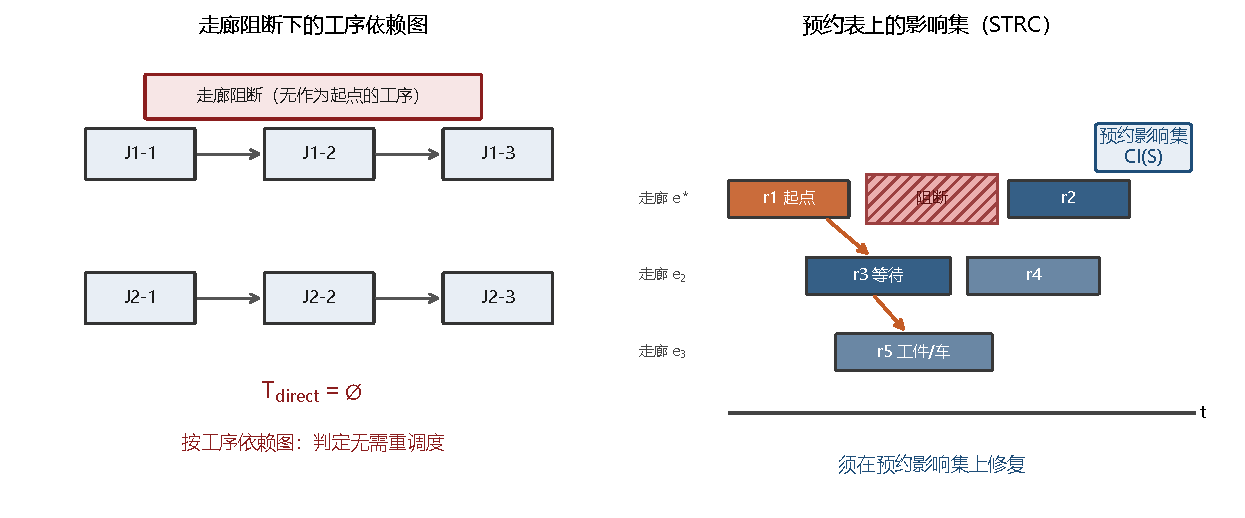
\includegraphics[width=\linewidth]{figures/fig_strc_motivate_CN}
\caption{动机示意。左:走廊阻断不使任何工序或机器无法按原计划执行,工序依赖图上没有作为起点的工序。
右:同一扰动下,与阻断时段重叠的走廊占用成为起点,并沿让行与接续关系形成预约影响集。}
\Description{并排两幅图。左幅是工序依赖图,走廊阻断没有使任何工序节点无法执行,
作为起点的工序集为空。右幅是同一时刻的走廊预约表,与阻断时段重叠的占用成为起点,
这些占用沿让行边与接续边向外连成一片传播区域。}
\label{fig:motivate}
\end{figure}

\subsection{本文主张}

本文有三点主张。

第一，当柔性作业车间用时间窗预约保证车辆无冲突通行时，扰动后的重调度范围应定义在由走廊占用及其让行关系构成的时空预约图上，而不是只定义在工序依赖图上。

第二，划界对象是时空预约闭包（\STRC, Spatiotemporal Reservation Closure），即预约影响集：
以与扰动时窗重叠、因而失效的走廊占用为起点，沿让行、同一车辆的后续占用、同一工件下一道工序的占用、同一机器上下一道工序的占用，
把直接或间接必须作废、重写的走廊占用全部收录。
这些依赖关系一经给定，影响集以外的占用不再是集内占用沿上述关系的下一步，
因而「改写哪些占用」对应一个可以检验的集合，而不是人为设定的搜索半径。

第三，得到影响集之后，在集内为原车改路、集外保持原占用；若仍得不到可行排程，
再按同一工件、同一车辆、直至全部未完成占用的顺序，扩大允许改写的范围。
A 类故障上另允许换车与改派，仍不改加工顺序。
这些步骤用来落实影响集并恢复可行排程；本文的主张在于如何划定影响集，而不在这些修复步骤是否新颖。

上述三点共用一个立场：\textbf{预约影响集是一次测量，不是一个决策。}
本文不用「谁挡了谁」去引导搜索以更换指派或路径——那是在改进排程决策；
消去一处走廊等待之后，另一处约束往往会成为新的瓶颈，完工时间上的收益因此容易被抵消。
本文用同一份「谁挡了谁」去划定哪些占用已经损坏：依赖关系给定后，
一条占用是否属于影响集，取决于它能否从起点沿这些关系到达，结果唯一确定，
不随之后哪一条约束成为新的瓶颈而改变。

这并不等于声称影响集已经包含物理上所有必须改写才能恢复可行的占用。
画哪些依赖边、不画哪些，是建模时的选择；边集一旦选定，
影响集对外封闭（集内占用没有指向集外的依赖边）就是该定义的推论
（命题~\ref{prop:struct}），不是另外证明出来的性质。
影响集是否为恢复可行所需的最小占用集合，本文不作主张：
最小集合依赖于允许哪些修复动作，而影响集刻意不绑死某一种修复方法
（注~\ref{rem:minimality}）。

相对以原排程为起点、在限定时间内重新搜索的全局重调度，预约影响集回答的是另一类问题：
在必须很快给出可执行方案时，能否恢复可行，并把改写限制在影响集以内。
修复后，影响集以外每条走廊占用的走廊、时段与车辆均与原计划一致——
这是边集给定、且集外占用已按原计划成功写入新表时的充分条件
（命题~\ref{prop:outside}），不是无条件成立的等式。
相对不改写决策时刻已经结束的占用的全局重调度，有界修复得到的完工时间 \(C_{\max}\) 更差，
两边被改写的占用比例已在同一量级；其长处在于算法耗时短得多（毫秒对秒）。
算法耗时与改写比例不应混在一处解释，第~\ref{sec:cheap}~节已分开测试：
耗时短来自对影响集内各段运输各做一次路径规划、不重开种群搜索，并不来自影响集本身；
至于影响集是否少改写了占用，不能从上述全局重调度对照中读出——两边比例已经接近——
而须另设一对照：改路程序相同，唯一差别是允许改写的是影响集，还是尚未结束的全部占用。
在测到的 \(6\) 个算例--随机种子格上，各搜索时限处全局重调度得到的 \(C_{\max}\) 都更小，未观察到有界修复反过来更优的情形。
因此，有界修复的作用不是降低完工时间，而是在毫秒内给出可执行的修复方案。
按工序依赖图划界时，走廊阻断因找不到受影响工序而不会启动局部重调度，原排程保持不可行。
同一扰动若改为启动全局重调度，则可以处理，但算法耗时在秒级。
当必须立刻恢复可行时，需要先识别走廊占用上的损坏范围，再选用与之匹配的局部恢复步骤。
本文解决的不是找到一种完工时间上更优的重调度算法，而是这件识别与恢复的事。

\subsection{贡献}
\label{sec:contributions}

本文的贡献如下。

\begin{enumerate}[leftmargin=1.6em,itemsep=0.4em]
\item \textbf{指认工序依赖图覆盖不到的一类损坏。}
当排程同时用工序依赖刻画加工先后、又用时间窗记录走廊占用时，
现成的重调度范围仍按受影响工序划定。
走廊阻断、走廊通行变慢等扰动不改任何工序指派，
按该方法划出的范围为空，并据此判为无需重调度；
但与受扰时段重叠的走廊占用已经失效，原排程不可行，
等待还会沿让行关系传给后续车辆。
这一缺口不是检测漏检，而是工序依赖图不含占用之间的让行关系；
运输时间若仍取为常数矩阵，走廊不是可争用资源，这类损坏甚至写不进模型。

\item \textbf{把重调度范围定义为预约影响集。}
以与扰动时窗重叠的走廊占用为起点，
沿让行、同一车辆的后续占用、同一工件与同一机器上下一道工序的占用，
收录直接或间接必须作废、重写的记录，得到时空预约闭包（\STRC）。
依赖关系一经给定，一条占用是否属于影响集唯一确定，
集内占用没有指向集外的依赖边，因而「改写哪些」对应一个可检验的集合，
而不是人为设定的搜索半径，也不随某一种改路算法如何实现而变。
影响集是一次测量，不是一个排程决策：本文用「谁挡了谁」划定损坏，
而不用它去引导搜索更换指派或路径。
本文不主张影响集已是恢复可行所需的最小占用集合
（最小集合依赖于允许哪些修复动作，注~\ref{rem:minimality}）。
\emph{这一层——影响集作为对象是否成立——的证据是}：走廊阻断下工序依赖图上的范围为空
而原排程确已不可行 \(\PassMiss\)（第~\ref{sec:e1}~节）、A 类上预约影响集不丢工序依赖图
已纳入的占用 \(\PassClosed\)
（第~\ref{sec:e2}~节）、边界消融的差分试探泄漏 \ProbeLeakPairs。
\emph{而划这条界在净收益上值不值，本文的证据只到 RA 这一档}（第~\ref{sec:cheap}~节）：
与"改写全部尚未结束的占用"相比少改写多少，两层不可混为一句。

\item \textbf{给出与该划界相匹配的局部恢复，并分清各项读数各来自何处。}
在影响集内为原车改路、集外保持原占用；仍不可行时再扩大允许改写的范围。
这些步骤用来落实影响集，本身不是本文的方法贡献。
在同一套走廊路网、时间窗路由与无冲突校验下对照表明：
按工序依赖图划界时走廊阻断 \(\FeasRone\) 恢复可行，按预约影响集划界时 \(\FeasRtwo\) 恢复可行，
可行与否来自划界对象，而不是改路程序的优劣；
有界修复以毫秒级耗时恢复可行，但完工时间 \(C_{\max}\) 较全局重调度更差，
且放宽预算不出现反超（\(\EfiveCells\) 个算例--随机种子格，所测预算区间内无交叉点）；
相对「改写全部尚未结束的占用」的对照，耗时与 \(C_{\max}\) 几乎不变，
少改写的占用才可归因于影响集（第~\ref{sec:cheap}~节）。
四类扰动与两种划界的交叉中，工序依赖图范围仅在走廊阻断与通行变慢上为空，
预约影响集均非空，且在机器或车辆故障上不小于工序依赖图范围。
\end{enumerate}

同一车间、同一预约表上，开工前的一体化排程用预约表构建无冲突方案~\cite{vanos2026exact,li2026framework,sun2023integrated}；
本文在执行时刻用预约表定位损坏范围。二者时机不同，并不互相替代。

\subsection{篇章结构}

第~\ref{sec:related_work}~节按四类回顾相关工作：作业车间如何按工序或时间轴划定重调度范围、
铁路调度如何表达排他资源上的占用先后、无冲突多车路径如何做局部重规划，
以及考虑运输的柔性作业车间把边界划在何处，并据此说明本文的位置。
第~\ref{sec:problem}~节给出走廊预约设定与执行期恢复问题：
车间、走廊预约表与工序依赖图，两类扰动，以及恢复须满足的条件。
第~\ref{sec:strc}~节定义时空预约闭包，即预约影响集，说明其依赖边与对外封闭等性质
（图~\ref{fig:graphs}、\ref{fig:closure}）。
第~\ref{sec:repair}~节说明如何在影响集内为原车改路、集外保持原占用，
以及仍不可行时如何扩大允许改写的范围，并与全局重调度对照（图~\ref{fig:framework}）。
第~\ref{sec:experiments}~节报告可行性、算法耗时、占用改写比例与完工时间，
并用案例甘特把统计结果落到工序时间轴上。
第~\ref{sec:conclusion}~节总结全文，并讨论局限与后续工作。

%% =====================================================================
\section{相关工作}
\label{sec:related_work}
%% =====================================================================

%% 相关工作按问题类型回顾,不作「四层定位」。旧文献以引文簇保留,叙述以近作为主。

动态调度的一个基本问题是：扰动发生后，重调度范围划在什么对象上，即改哪些、其余保持不动。
已有文献把这一范围划在不同对象上——工序或时间轴、排他资源上的占用先后、
受影响的车辆，以及带运输的柔性作业车间中的工序集合。
下面按这四类回顾各自做了什么、尚未覆盖什么，并在表~\ref{tab:position} 中做汇总。

\subsection{作业车间的局部重调度}
\label{sec:rw_aor}

对机器故障、插单等工序事件,按受影响工序划定重调度范围,在带 AGV 的动态调度中仍被采用。
Zhang 等~\cite{zhang2023energy} 处理机器故障与插单,恢复范围取故障后尚未加工的工序;
Tang 等~\cite{tang2026dynamic} 按扰动传播把工序与配送任务分为保留、继续、重构,
并把完全重调度、部分重调度与右移并列,指出右移保住稳定性、让出优化空间。
这一做法可上溯至受影响工序重调度(AOR)~\cite{abumaizar1997rescheduling,subramaniam2003maor}:
只重排被扰动直接或间接波及的工序。
沿时间轴划界与失败后扩大范围同样已有文献研究过,包括 match-up~\cite{akturk1999matchup}
与增量扩大时间窗的 Local Rescheduling~\cite{kuster2007local}。
右移则不判定谁受影响,把未完成部分整体后推。
滚动时域与分解式方法在规模与质量之间折中~\cite{zeitrag2025novel,zhao2019decomposition};
综述见~\cite{vieira2003rescheduling,ouelhadj2009survey}。

这些工作表明,划定范围再局部重调度并不是新问题,前提是扰动首先作用在工序上。
一旦扰动只使走廊不可通行而不改指派,按该方法划出的范围可以为空,原排程却已不可行。

\subsection{排他资源上的占用先后}
\label{sec:rw_ag}

「谁先占用同一排他资源」被建成图,在铁路调度中已有系统研究。
Mascis 与 Pacciarelli~\cite{mascis2002alternative} 的 alternative graph
把析取图推广为:顶点是作业对闭塞区段的占用,固定弧表示路径先后,
成对的 alternative arc 表示谁先通过该区段。
D'Ariano 等人~\cite{dariano2007branch} 用该模型做列车实时重调度,
扰动后重算无冲突时刻表,并尽量接近原计划。
同走廊上的让行关系与 alternative arc 表达的是同一类先后。

与本文不同的是用法。对每一处争用，alternative graph 给出两条互斥的弧
（甲先通过，或乙先通过），排程就是从中选定一条：
选定后图中不能出现正权回路，时刻表才可行，并尽量使目标最优——占用先后因此是决策变量。
本文的计划已经排好，谁先通过哪条走廊已经确定，不再选择先后，
只按这些既定的让行与接续关系，把扰动后必须作废的原走廊占用纳入重调度范围。
此外,铁路模型把闭塞区段当作机器,工序与占用在同一张图上,
区段不可用就是工序事件,不存在「范围画在工序依赖图上、因而漏掉走廊阻断」。
柔性作业车间里加工与走廊占用是两套对象,现成的 AOR 划界用不上这一套占用先后。

\subsection{无冲突多车路径的局部重规划}
\label{sec:rw_mapf}

在多智能体路径规划中,只为受影响者进行重调度、其余视为动态障碍,已是标准做法。
Švancara 等人~\cite{svancara2019online} 在在线 MAPF 中给出
Replan All、Replan Single 与 Replan Affected,并用在线独立性检测确定受影响集合;
Malka 等人~\cite{malka2024online} 在地图不准确时,同样只为受观测变化影响的车辆重规划。
无冲突路径规划把时空占用作为一等约束,但起终点通常由外部给定~\cite{zhang2024guidance}。

上述做法已经把「只改受影响者、其余保持原计划」做成标准机制，本文并不把它当作贡献。
与本文设定的另一点不同是：这类工作只有车辆的起终点，没有工件—工序—机器指派，
因而不会出现「重调度范围按工序依赖图划定，走廊阻断因找不到受影响工序而被漏掉」。
就受影响集合如何得到而言，MAPF 用独立性检测找出受影响车辆，得到的是检测算法的输出，随实现方式和停止条件而变。
本文给出的预约影响集则不同：依赖边一经给定，一条占用是否属于该集，
只取决于它能否从起点沿这些边到达，与随后用哪一种改路算法无关
（第~\ref{sec:containment}~节）。

\subsection{考虑运输的柔性作业车间调度}
\label{sec:rw_position}

考虑运输车辆的柔性作业车间调度已有系统综述~\cite{xin2025review}。
近期组合优化工作仍普遍把行驶时间取为按位置对索引的常数矩阵,
并在此之上发展约束规划、元启发式与知识引导搜索~\cite{meng2025cp,qin2026knowledge,fu2025integrated}。
该约定下车辆并不争用同一路段,走廊阻断在模型里没有对应对象,无法被检验。

一旦用时间窗记录走廊占用,加工先后与走廊占用同时进入模型。
拥堵感知派车可用局部密度等代理量选车,而不改机器指派~\cite{kim2026congestion}。
把柔性指派与无冲突运输真正合在一起的工作相对较少:
van Os 与 Basten~\cite{vanos2026exact} 形式化了带无冲突运输约束的柔性作业车间调度,
并以分解方法在多数基准算例上取得可证最优,少数因限时未能保证最优性;
两阶段方案先固定排产再消解车辆冲突~\cite{sun2023integrated};
亦有学习层排产、路径层消冲突、并以有限反馈连接的框架~\cite{li2026framework}。
但这些工作回答的是开工前如何排出可行且质量好的无冲突排程。

据作者所知,尚未见到同时纳入走廊预约表与执行期扰动响应的工作。这一句是有限度的:
本文不声称已穷尽文献,因而不把它写成全称否定。可逐篇核对的事实是,
在本节所引的这些工作里两个条件没有同时出现——有预约表的把执行期故障排除在外,
处理执行期扰动的则没有预约表。
以下两处是直接引原文假设的:
Zhang 等~\cite{zhang2023energy} 在建模假设中写明忽略 AGV 之间的碰撞；
Sun 等~\cite{sun2023integrated}
用时间窗 Dijkstra 消解车辆冲突,却在假设中写明不考虑车辆的充电与故障、车辆始终可用,
并把设备维护与故障列为后续研究。

因此,缺口不是某篇已有文献把边界画错了,而是在上列工作中两个条件没有同时到位:
工序级划界成立,往往因为没有走廊预约;已有预约表的设定,又把执行期扰动排除在外。
一旦两者同时出现,现成可沿用的只有按受影响工序划界的做法,
它对不改工序指派的走廊阻断会给出空范围(第~\ref{sec:e1}~节实测 \PassMiss)。
本文要处理的就是这一情形。需说明的是,\textbf{该反例本身不依赖上述缺口陈述成立}:
即便已有工作同时纳入了两个条件,第~\ref{sec:e1}~节的读数仍然成立,
受影响的只是本文的新颖性主张,不是它的正确性。

\subsection{本文定位}
\label{sec:rw_claim}

\begin{table*}[t]
\centering
\caption{相关工作按\emph{划界对象}分类:每类工作把扰动后"需要改写什么"定义在哪种对象上。
「边界划在」为重调度范围所依附的对象;「有工序依赖图?」兼答该图是否与占用同图;
末行加粗者为本文所处的类别。}
\label{tab:position}
\small
\begin{tabular}{@{}p{0.16\linewidth}p{0.22\linewidth}p{0.14\linewidth}p{0.14\linewidth}p{0.24\linewidth}@{}}
\toprule
\textbf{类别} & \textbf{代表工作} & \textbf{边界划在} & \textbf{有工序依赖图?} & \textbf{与本文的关系} \\
\midrule
作业车间局部重调度 &
AOR~\cite{abumaizar1997rescheduling,subramaniam2003maor};
match-up~\cite{akturk1999matchup};
LRS~\cite{kuster2007local};
带 AGV 的动态调度~\cite{zhang2023energy,tang2026dynamic} &
工序 / 时间窗 & 有 &
后文对照复现按工序划界与右移 \\
\addlinespace[2pt]
排他资源占用先后 &
alternative graph~\cite{mascis2002alternative};
铁路实时重调度~\cite{dariano2007branch} &
闭塞区段占用 & 有,与占用在同一张图 &
让行关系同类；铁路用它选择车辆的先后，本文用既定先后划定需要改写的占用 \\
\addlinespace[2pt]
无冲突多车路径 &
Online MAPF~\cite{svancara2019online,malka2024online};
LMAPF~\cite{zhang2024guidance} &
受影响车辆 & 无 &
集内改路、集外保持已是标准做法 \\
\addlinespace[2pt]
带运输的柔性作业车间 &
常数矩阵~\cite{xin2025review,meng2025cp,qin2026knowledge,fu2025integrated};
一体化排程~\cite{vanos2026exact,sun2023integrated,li2026framework} &
工序集合 & 有;预约表与执行期扰动未同时出现 &
\textbf{本文的位置} \\
\bottomrule
\end{tabular}
\end{table*}

综上，在考虑 AGV 无冲突路由的柔性作业车间中，排程同时用工序依赖刻画加工先后，
又用时间窗记录走廊占用。此时会出现前节所指缺口对应的情形：
走廊阻断等扰动并不使工序无法执行，原指派仍然有效，
但与受扰时段重叠的走廊占用已经失效，原排程不可行。
后文按工序依赖图划界的对照，复现的是第~\ref{sec:rw_aor}~节的做法。
本文主张把重调度范围改到走廊占用及其让行、接续关系上，得到由这些关系唯一确定的预约影响集。

%% =====================================================================
\section{走廊预约设定与执行期恢复问题}
\label{sec:problem}
%% =====================================================================

\subsection{系统设定与记号}
\label{sec:system_brief}

问题设定沿用带无冲突运输约束的柔性作业车间~\cite{vanos2026exact}。
本节一次写清后文用到的对象。一份可行排程 \(\mathcal{S}^0\) 视为给定输入:
它在 \(t=0\) 如何被搜索出来,不影响后文如何划定须改写的占用。

\subsubsection{车间与四组决策}
\label{sec:shop}

车间路由图 \(G=(V,E)\) 强连通。机械臂占据固定节点 \(\mathrm{loc}(m)\);
\(v_0\in V\) 为装卸站。\(n\) 个工件、机器集合 \(M\)、同构单载车队
\(K=\{1,\ldots,N_A\}\)。工件 \(j\) 有固定工序链 \(O_{j1}\to\cdots\to O_{jn_j}\);
工序 \(O_{ji}\) 的候选机器集为 \(\Omega_{ji}\subseteq M\),在机器 \(m\) 上耗时
\(t^P_{jim}\)。一份完整排程同时确定四组决策:
(i)~每道工序的机器指派 \(x\);
(ii)~各机器上的工序扫描序 \(\pi\);
(iii)~各次搬运的车辆指派 \(y\);
(iv)~每次车辆移动在 \(G\) 上的无冲突路径。
记
\[
\mathcal{S}=(x,\,\pi,\,y,\,R),
\]
其中预约表 \(R\) 是第 (iv) 组的显式记录,定义见下。

运输任务由指派\emph{派生},不是输入:仅当相邻两道工序不在同一节点时才产生一次搬运。
一次搬运拆成两段——空载取货与满载送达——各段有自己的任务标签 \(u\)
(例如 \(O_{ji}\) 的空载段与满载段是两条记录)。装卸取瞬时:满载段在空载段抵达与工件就绪
二者中较晚的时刻起行,而送达时刻同时就是机器可开工、车辆可接新任务的时刻。
后文允许改写哪些占用、哪些占用保持原计划,以及如何改路,都以段为粒度,而不是整道工序。

\subsubsection{走廊预约与无冲突}
\label{sec:reservation}

每条走廊 \(e\in E\) 是排他资源,通行时间 \(\tau_e\) 已知;两个方向共享同一份占用,
因而任一时刻至多一辆车占用 \(e\),迎面冲突与同向超车一并排除。
占用取半开区间:第二辆车可以恰好在区间右端点进入。
节点上设容量充裕的停靠位,等待发生在节点上且总是被允许。
一条预约记录为
\[
r=(e,\,[t^s,t^e),\,k,\,u)\in R,
\]
即车辆 \(k\) 在 \([t^s,t^e)\) 占用走廊 \(e\),所属运输段为 \(u\)。
同一走廊上任意两次不同占用必须满足
\([t^s,t^e)\cap[t^{s\prime},t^{e\prime})=\varnothing\)。
路径只写入 \(R\) 报告为空闲的时窗,故无冲突是构造出来的,不是事后修补的。

时间窗路由是后文改路与各对照方法共用的原语:给定起终点、最早出发时刻与当前 \(R\),
它返回一条与已有占用无交的通路及各走廊进入时刻。
实现上采用时间窗 Dijkstra~\cite{sun2023integrated};本文不改这条原语,
只改\emph{哪些}运输段被送进路由器。
与 van Os 预约节点、Lyu 另加节点容量不同~\cite{vanos2026exact,lyu2019approach},
本文预约的是边;第~\ref{sec:limitations}~节交代由此带来的算例口径限制。

\subsubsection{工序依赖图与预约依赖图}
\label{sec:two_graphs}

工序依赖图 \(G_T=(T_T,E_T)\)(文献中亦称任务图,下标 \(T\) 取自 task)以工序为顶点,
边为工件先后与同机先后;
它\emph{不含}走廊占用之间的让行关系。
预约依赖图 \(G_R=(R,E_R)\) 以 \(R\) 中的占用为顶点,边为让行、同车、同工件与同机所诱导的依赖
(定义~\ref{def:dep})。
两张图的顶点集不相交:一边是加工,一边是通行。
因此存在一类只改走廊时窗、不改任何工序参数的扰动——按 \(G_T\) 划界时找不到作为起点的工序,
而按 \(G_R\) 划界时起点占用非空,且原排程已不可行。
图~\ref{fig:graphs} 对照这两张图;图~\ref{fig:motivate} 给出走廊阻断下的后果;
表~\ref{tab:notation} 汇总本节及后文用到的记号。

\begin{figure}[t]
\centering
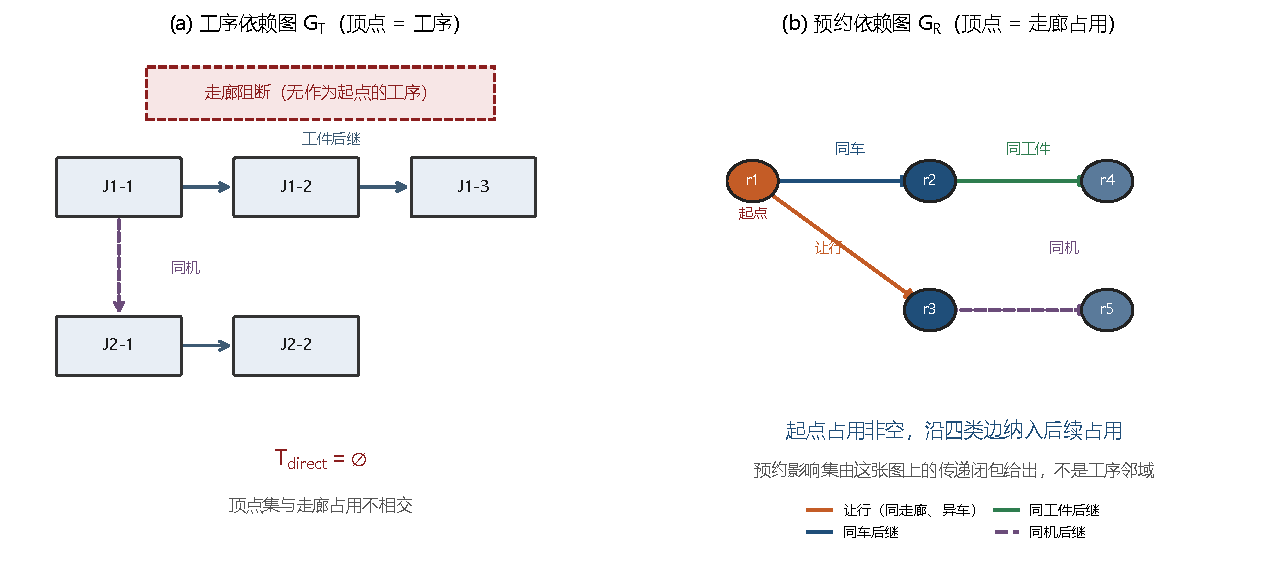
\includegraphics[width=\linewidth]{figures/fig_strc_graphs_CN}
\caption{两张图的顶点集不相交(构造示意)。
(a)~工序依赖图 \(G_T\),顶点是工序,走廊阻断找不到作为起点的工序;
(b)~预约依赖图 \(G_R\),顶点是走廊占用,从与阻断窗重叠的占用出发,沿四类依赖边
(让行、同车、同工件、同机;定义~\ref{def:dep})纳入后续占用。}
\Description{并排两幅。左幅是工序依赖图,工件后继与同机后继连在工序方框之间,
顶部一条虚线框标出走廊阻断,阻断没有落在任何方框上。
右幅是预约依赖图,五个圆形顶点表示走廊占用,四条不同颜色的箭头分别标为
让行、同车、同工件与同机。}
\label{fig:graphs}
\end{figure}

\begin{table}[t]
\centering
\caption{本文常用记号}
\label{tab:notation}
\small
\begin{tabular}{@{}ll@{}}
\toprule
\textbf{符号} & \textbf{含义} \\
\midrule
\(G=(V,E)\), \(\tau_e\) & 走廊路网;走廊 \(e\) 的通行时间 \\
\(v_0\), \(\mathrm{loc}(m)\) & 装卸站;机械臂 \(m\) 所在节点 \\
\(x,\pi,y\) & 机器指派、扫描序、车辆指派 \\
\(R\), \(r=(e,[t^s,t^e),k,u)\) & 预约表;一条半开占用(车辆 \(k\),段标签 \(u\)) \\
\(G_T\) / \(G_R\) & 工序依赖图 / 预约依赖图 \\
\(\mathcal{S}^0,\mathcal{S}'\) & 扰动前排程、恢复后排程 \\
\(\mathcal{D},\,t_{\mathrm{now}}\) & 扰动事件、发生(决策)时刻 \\
\(T_{\mathrm{direct}},\,T_{\mathrm{impact}}\) & 工序依赖图上直接受扰的工序 / \(\theta\)-步纳入范围 \\
\(\mathrm{Seeds}(\mathcal{D})\), \(U\) & 作为起点的占用;允许改写的占用集合 \\
\(\mathrm{Cl}(\cdot)\) & 预约影响集(\STRC) \\
\(\varphi\) & 受扰未来工序比例(规模扫描) \\
\bottomrule
\end{tabular}
\end{table}

\subsection{执行期假设}
\label{sec:assumptions}

执行期约定与物理设定如下。其中 A1--A4 由全部对照方法共用,以便把读数归因到重调度范围
如何划定,而不是模型差异;A5 只约束本文方法,全局重调度对照的允许动作更宽(见该条末句):

\begin{enumerate}[label=\textbf{A\arabic*.},leftmargin=*,topsep=2pt,itemsep=2pt]
\item \textbf{初始排程可行。} \(\mathcal{S}^0\) 在扰动前通过无冲突校验;预约表与工序时间表一致。
\item \textbf{已完成占用不回溯。} 只改写 \(t_{\mathrm{end}}>t_{\mathrm{now}}\) 的未来占用
与未完工工序; \(t_{\mathrm{end}}\le t_{\mathrm{now}}\) 的占用字段不可改写。
\item \textbf{单次、完全观测。} 扰动在 \(t_{\mathrm{now}}\) 被完整观测,且不与其它扰动叠加;
扰动流、预测误差与滚动响应不在本文范围内。
\item \textbf{走廊排他、缓冲充裕、车队同构单载。} 走廊仍为排他半开资源,阻断以附加占用
(或禁行窗)注入路由层。有限缓冲、充电、加减速与装卸时长不建模;
全部车辆在计划开始时空载停于 \(v_0\)。
\item \textbf{允许的恢复动作。} B 类扰动保持原机器指派 \(x\) 与扫描序 \(\pi\),只改路;
失败时扩大允许改写的占用集合。A 类故障额外允许:车辆故障把故障车从车队摘除并换车;
机械臂故障把未完工工序改派到其它可行机。扫描序 \(\pi\) 始终不变,不重开搜索。
实验中的全局重调度对照可以改 \(x\) 与 \(\pi\)(第~\ref{sec:vs_r0}~节)。
\end{enumerate}

\subsection{扰动二分}
\label{sec:disturbance_classes}

\begin{definition}[A/B 类扰动]
\label{def:ab}
若扰动直接使某些工序的指派或\emph{可执行性}失效(机械臂故障、显著工时偏差、插单、
车辆故障等),称其为 \textbf{A 类};若扰动只使某些走廊时窗不可用、而不使任何工序
不可执行(走廊阻断、走廊通行变慢等),称其为 \textbf{B 类}。
\end{definition}

\begin{remark}[车辆故障为何属于 A 类]
\label{rem:agv_class}
车辆故障不改动任何工序的机器指派,乍看应与走廊阻断同类。但定义~\ref{def:ab} 的判据是
\emph{可执行性}而非指派:一辆车抛锚后,它承运的那些工序在原计划下无法开工,
故经「车辆\(\to\)所承运工序」的映射,工序依赖图上仍有作为起点的工序。这一归类把车辆故障
划到按工序划界能够给出非空范围的一侧。
只有当重调度方法维护了车--任务映射时,这些起点工序才非空;若方法只跟踪工序与机器
(AOR 的常见实现即如此),车辆故障同样会得到空范围。本文不依赖这一点立论,
第~\ref{sec:e6}~节按维护了该映射的强口径报告 A 类读数。
\end{remark}

\begin{definition}[工序依赖图上的直接集与影响域]
\label{def:task_impact}
对扰动 \(\mathcal{D}\),令 \(T_{\mathrm{direct}}(\mathcal{D})\) 为因机器故障、车辆故障或工序失效
而无法按原计划执行的工序集合。对 B 类走廊扰动约定 \(T_{\mathrm{direct}}=\varnothing\)。
在 \(G_T\) 上从 \(T_{\mathrm{direct}}\) 出发,按工件后继与同机后继纳入深度至多 \(\theta\) 的工序,
记为 \(T_{\mathrm{impact}}(\mathcal{D},\theta)\)。
\end{definition}

\begin{definition}[作为起点的占用]
\label{def:seeds}
起点集 \(\mathrm{Seeds}(\mathcal{D})\subseteq R\) 按扰动类型给出,一律只取
\(r.t^e>t_{\mathrm{now}}\) 的占用。
\begin{enumerate}[label=(\alph*),leftmargin=1.6em,itemsep=0.15em]
\item \textbf{走廊阻断/降速} \(\mathcal{D}=(e,[t_a,t_b))\):
\(\{\,r:\ r.e=e,\ [r.t^s,r.t^e)\cap[t_a,t_b)\neq\varnothing\,\}\)。
多处短暂阻断时取各窗起点占用之并。两者共用这条起点规则(原排程按时长未缩放的 \(\tau\) 写出,
与窗重叠的占用都已失效),故划定须改写的占用时二者给出同一个预约影响集——第~\ref{sec:e6}~节据此说明
为何不把二者的划界读数算作两次独立验证;改路时二者已分开,降速只缩放与窗重叠的
那一段进度,而不再写成整段禁行,也不再把有交的穿越整段乘倍率。
\item \textbf{车辆故障} \(\mathcal{D}=(k)\):该车在 \(t_{\mathrm{now}}\) 之后的全部占用
\(\{\,r:\ r.k=k\,\}\)。
\item \textbf{机械臂故障} \(\mathcal{D}=(m,F)\),\(F\) 为该机上尚未完工的工序:
对每个工件取 \(F\) 中最小工序号 \(i_{\min}(j)\),起点占用为各工件自该工序起(含)的全部
未来占用。之所以沿工件链向后取而不只取该工序自身,是因为进站运输可能已在
\(t_{\mathrm{now}}\) 前结束,若只取自身,预约影响集会短于工序依赖图上的影响域,对照即不公平。
\end{enumerate}
\end{definition}

\begin{prop}[B 类上工序依赖图给出空范围]
\label{prop:miss}
设 \(\mathcal{D}\) 为走廊阻断。若采用定义~\ref{def:task_impact} 对 B 类的约定,则
\(T_{\mathrm{direct}}(\mathcal{D})=\varnothing\),从而对任意有限 \(\theta\ge 0\) 有
\(T_{\mathrm{impact}}(\mathcal{D},\theta)=\varnothing\)。
若此外 \(\mathrm{Seeds}(\mathcal{D})\neq\varnothing\),则 \(\mathcal{S}^0\) 在 \(\mathcal{D}\) 下不可行。
\end{prop}

\begin{proof}
走廊阻断只使走廊时窗不可用而不使任何工序不可执行,故按定义~\ref{def:ab} 属 B 类。
这一步用到两条前提:阻断窗 \([t_a,t_b)\) 有限,且由假设 A4 缓冲充裕,车辆可在窗外通行;
因而即使阻断期内路网被割断,也没有工序变得不可执行,只是被推迟。若阻断无限期、
或缓冲不足以支持等待,该扰动按定义~\ref{def:ab} 就该归 A 类,不在本命题范围内。
既属 B 类,
再由定义~\ref{def:task_impact} 对 B 类的约定,\(T_{\mathrm{direct}}=\varnothing\)。
\(\theta\)-步纳入的起点为空,故 \(T_{\mathrm{impact}}=\varnothing\)。
若存在 \(r\in\mathrm{Seeds}(\mathcal{D})\),则 \(r\) 的占用区间与禁行窗相交。
将 \(\mathcal{D}\) 解释为该走廊上的强制占用后,\(r\) 与禁行窗在同一排他资源上时间重叠,
违背半开时窗无冲突条件(假设 A4 的走廊排他),故 \(\mathcal{S}^0\) 不可行。
\end{proof}

命题~\ref{prop:miss} 是问题层面上的反例。前半句由定义~\ref{def:task_impact} 对 B 类的约定直接得到
(工序依赖图按定义不含走廊占用之间的让行关系,因而覆盖不到走廊阻断);
非平凡的是后半句——起点占用非空时原排程已经不可行,
因而「工序依赖图上范围为空白 \(\Rightarrow\) 无需重调度」在用时间窗预约走廊的设定下不成立。
该反例不依赖任何修复算法;实验第~\ref{sec:experiments}~节给出算例规模。

\subsection{恢复问题}
\label{sec:recovery_problem}

\begin{problem}[按预约表划定范围的有界恢复]
\label{prob:recovery}
给定可行排程 \(\mathcal{S}^0\)、扰动 \(\mathcal{D}\) 与时刻 \(t_{\mathrm{now}}\),
求 \(\mathcal{S}'\),使得:
(i)~\(\mathcal{S}'\) 在 \(\mathcal{D}\) 下通过无冲突校验;
(ii)~未纳入改写范围的占用,其走廊、时段与车辆尽可能与 \(\mathcal{S}^0\) 一致;
(iii)~算法耗时受预算约束。
次级目标为完工时间 \(C_{\max}(\mathcal{S}')\)。
\end{problem}

求解拆为两步:先划定允许改写的占用集合 \(U\subseteq R\);
再只对 \(U\) 内运输改路,集外占用保持原计划。
本文用 \(\mathrm{Cl}(\mathrm{Seeds})\) 给出 \(U\);对照则用工序依赖图上的影响域诱导出预约子集。

%% =====================================================================
\section{时空预约闭包}
\label{sec:strc}
%% =====================================================================

本节只产出允许改写的占用集合 \(U\):输入预约表 \(R\) 与起点占用集 \(\mathrm{Seeds}(\mathcal{D})\)
(定义~\ref{def:seeds}),在占用之间建依赖图并取传递闭包,输出 \(U=\mathrm{Cl}(\mathrm{Seeds})\);
在 \(U\) 上如何改路属第~\ref{sec:repair}~节。

\subsection{预约依赖边}
\label{sec:closure_def}

\begin{definition}[预约依赖图]
\label{def:dep}
顶点为 \(R\) 中的走廊占用。有向边 \(r\to r'\) 表示「\(r\) 失效可能迫使 \(r'\) 改路」,包括:
\begin{enumerate}[leftmargin=1.4em,itemsep=0.15em]
\item \textbf{让行边:} 同走廊、异车、时间重叠\emph{或半开区间接壤}
(\(r.t^e=r'.t^s\)),且先进入者指向后进入者;接壤在排他语义下合法,但前者延后则后者必须让路;
\item \textbf{同车后继:} 同一车辆按时间序相邻的两条占用;
\item \textbf{同工件后继:} 同一工件工序 \(i\) 的占用指向工序 \(i+1\) 的占用;
\item \textbf{同机后继:} 同一机器时间轴上相邻两道工序所诱导的占用之间的边。
\end{enumerate}
由此得到 \(G_R=(R,E_R)\)。
四类边的示意见图~\ref{fig:graphs}(b)。同工件后继连的是相邻工序所诱导的占用,
同机后继连的是同一机器时间轴上相邻两道工序所诱导的占用;
二者都以段为端点,与第~\ref{sec:shop}~节的粒度一致。
四类边只回答一个问题:\(r\) 改写之后 \(r'\) 是否可能必须跟着改。它们不试图刻画全部物理耦合,
边集本身是建模选择,其完备性由第~\ref{sec:e3}~节的差分试探检验,
相应限定见第~\ref{sec:containment}~节。
\end{definition}

\begin{definition}[\STRC{}]
\label{def:strc}
对起点占用集 \(S\subseteq R\)、视界 \(H\) 与时刻 \(t_{\mathrm{now}}\),
记决策时刻尚未结束、且开始时刻早于视界的占用为
\[
R^{\circ}=\bigl\{\,r\in R:\ r.t^e>t_{\mathrm{now}},\ r.t^s<H\,\bigr\},
\]
并令 \(G_R^\circ\) 为 \(G_R\) 在 \(R^{\circ}\) 上的诱导子图。
预约影响集（时空预约闭包）定义为
\[
\mathrm{Cl}(S)
=\bigl\{\,v\in R^{\circ}:\
\exists\,s\in S\cap R^{\circ}\ \text{使}\ s\!\to^*\!v\ \text{于}\ G_R^\circ\,\bigr\},
\]
即从尚未结束的起点占用出发,沿出边可达的全部尚未结束的占用(含起点自身)。
本文全部实验取 \(H=C_{\max}(\mathcal{S}^0)+1\),此时 \(r.t^s<H\) 对 \(\mathcal{S}^0\) 中每条占用
都成立、视界不起筛选作用,保留 \(H\) 只为使定义可用于滚动视界。
若以邻接表表示 \(G_R^\circ\)(记其边集为 \(E_R^{\circ}\)),则可用队列在
\(O(|R^{\circ}|+|E_R^{\circ}|)\) 时间内算出;该界未单独计时,
划界只是第~\ref{sec:cheap}~节毫秒档读数的一个组成部分。
\end{definition}

图~\ref{fig:closure} 给出示意:(a) 阻断窗与作为起点的占用;(b) 依赖边与预约影响集的外壳——
集外占用不是集内占用的出边后继(命题~\ref{prop:struct})。

\begin{figure}[t]
\centering
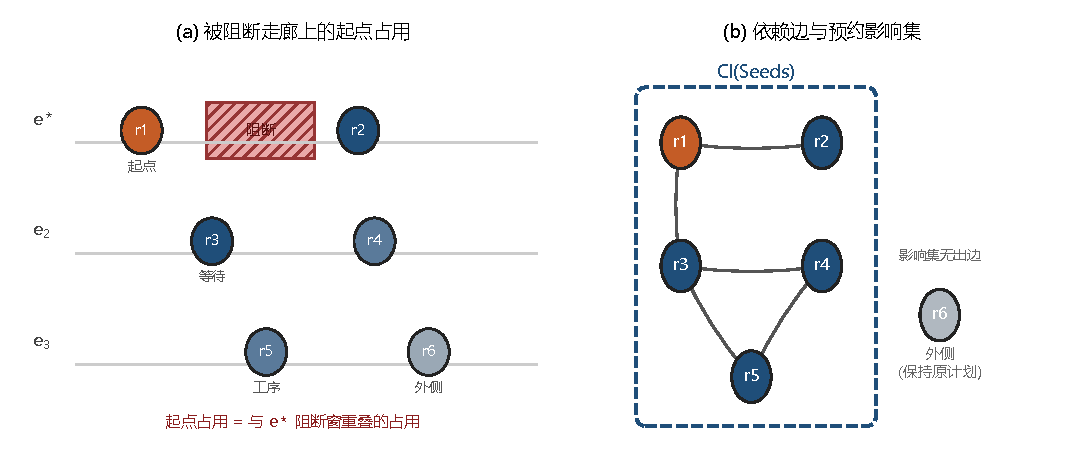
\includegraphics[width=\linewidth]{figures/fig_strc_closure_CN}
\caption{预约影响集的构造示意。
(a)~与走廊阻断窗重叠的占用作为起点;
(b)~沿四类依赖边(让行,以及同车、同工件、同机三类接续)取传递闭包得到
\(\mathrm{Cl}(\mathrm{Seeds})\),集外占用保持原计划。}
\Description{两小幅示意图。(a) 时空图上一段阻断窗覆盖若干条占用,
这些占用被标为起点。(b) 从起点沿有向依赖边做传递闭包,得到预约影响集的外壳;
外壳之外的占用没有来自壳内的入边,保持原计划。}
\label{fig:closure}
\end{figure}

按工序依赖图划界的对照,把 \(T_{\mathrm{impact}}\) 映射为允许改写的占用:
凡任务标签属于该影响域且 \(t^e>t_{\mathrm{now}}\) 的占用。
由命题~\ref{prop:miss},B 类上该集合为空。
按预约影响集划界时取 \(U=\mathrm{Cl}(\mathrm{Seeds})\)。
实验表中二者分别记为 R1 与 R2。

\subsection{包含性}
\label{sec:containment}

\begin{prop}[结构闭合性]
\label{prop:struct}
对任意 \(S\subseteq R\),在 \(G_R^\circ\) 中不存在边
\(u\to v\) 满足 \(u\in\mathrm{Cl}(S)\) 且 \(v\in R^{\circ}\setminus\mathrm{Cl}(S)\)。
因而,从 \(\mathrm{Cl}(S)\) 出发沿出边无法到达影响集外、尚未结束的占用。
\end{prop}

\begin{proof}
若存在这样的边 \(u\to v\),则由 \(u\in\mathrm{Cl}(S)\) 知存在尚未结束的起点占用 \(s\) 使
\(s\to^* u\)。拼接 \(u\to v\) 得 \(s\to^* v\),故按定义~\ref{def:strc} 应有
\(v\in\mathrm{Cl}(S)\),矛盾。
\end{proof}

命题~\ref{prop:struct} 说明「局部」对应一个图论上闭合的对象:影响集外的占用不是任何
集内占用的直接后继。这并不声称 \(G_R\) 已枚举物理世界中一切可能耦合——
边集是建模选择;一旦边集固定,闭合性就是定义的推论,而不是启发式半径。

\begin{remark}[预约影响集与最小允许改写集合]
\label{rem:minimality}
结构闭合性说明影响集足够大:集内占用没有指向集外的依赖边。
它并不说明影响集不过大。理由有三。

其一,\textbf{最小允许改写集合依赖于所用的修复程序,而预约影响集不依赖}。
称集合 \(U\) 为最小,须指明「在何种修复能力下 \(U\) 足以恢复可行」。允许改派与改序时的最小 \(U\),
与只允许改路时的最小 \(U\) 不是同一个集合。预约影响集由 \(G_R\) 唯一确定,与修复程序无关——
因而它在定义上不绑死某一启发式,也无法同时成为那种依赖修复程序的最小集。

其二,\textbf{四类边在充分方向仍是过近似;必要方向上,已知的那条接壤通道已经补上}。
让行边按「同走廊、异车、重叠或接壤」建立,只要重叠即连边,而不判断后者是否\emph{真的}
只能靠等待前者通过——若该处另有旁路,后者改道即可,本不必纳入允许改写的集合;同车后继边同样
可能把延误传不到的链尾一并纳入。这两处仍使影响集偏大。
接壤一度是反方向的漏边:半开区间首尾相接合法,旧规则不连边,但前者延后则后者必须让路。
现已并入让行边;差分试探在 \(\NPairs\) 对上泄漏为 \ProbeLeaks(\ProbeLeakPairs;
第~\ref{sec:limitations}~节)。这只关闭了这一条已观测到的通道,不是边集完备的证明。

其三,\textbf{实测上影响集并不小}。第~\ref{sec:e6}~节报告,走廊阻断下预约影响集平均覆盖
\(t_{\mathrm{now}}\) 之后尚未结束占用的约 \(90\%\);换言之,相对「把决策时刻尚未结束的占用全部纳入改写」这一平凡
上界,影响集少纳入的不足一成。有界修复真正省下的是\emph{不改写已经结束的占用}与\emph{不重开搜索},
而不是把未来切得很小。这一点在第~\ref{sec:e5}~节与局限一节中再次点明,
不应被「局部」「有界」这两个词读成「只动很小一块」。

「不足一成」是允许改写集合的\emph{规模}之比,不等于改写比例之差。
第~\ref{sec:cheap}~节把上述平凡上界作为一条独立对照(RA)实测后发现,正是这不足一成的
差别,把改动比例从 \ResFracAllFuture\ 降到 \ResFracCheapRtwo(逐格 \RAStabWTL,
\(p=\RAStabP\)),而算法耗时与完工时间几乎不变。

因此,本文给出的是由结构唯一确定、可复现、\emph{足以}恢复可行的允许改写集合,
并附带闭合性;逼近最小允许改写集合是另一个问题,列为后续工作
(第~\ref{sec:future}~节)。
\end{remark}

\begin{prop}[外侧字段不变的充分条件]
\label{prop:outside}
设允许改写的占用集合 \(U=\mathrm{Cl}(S)\),并设第 1 级改路按第~\ref{sec:level1}~节执行:
(i)~禁行窗已写入路由层;(ii)~对每个 \(r\in R^{\circ}\setminus U\),将其原字段
\((e,[t^s,t^e),k)\) 预提交到新预约表且预提交成功;
(iii)~仅对 \(U\) 内运输调用路由器生成新占用;(iv)~最终排程通过无冲突校验。
则在恢复后的预约表 \(R'\) 中,每条 \(r\in R^{\circ}\setminus U\) 的走廊、时段与车辆与
\(\mathcal{S}^0\) 一致。此处量词是逐\emph{占用}而非逐任务:一道运输可能一部分占用在 \(U\) 内、
另一部分在外,那时只有集外那部分受本命题保护。
\end{prop}

\begin{proof}
由 (ii),集外占用在重放开始前已按其原区间写入新表,且未与禁行窗冲突
(否则预提交失败)。步骤 (iii) 只为 \(U\) 内任务提交新占用,不删除或改写已提交的
集外区间。因此,对集外任务标签,新表中的 \((e,[t^s,t^e),k)\) 与预提交值相同,
亦即与 \(\mathcal{S}^0\) 相同。校验通过仅排除新占用与既有占用冲突,不改变已提交字段。
\end{proof}

前提 (i)--(iv) 是第~\ref{sec:level1}~节改路程序的执行条件,可对算法逐条核验,
与 A1--A5 那种模型级假设不同类,故不并入编号假设体系;命题此外依赖
A1(初始排程可行,否则集外原字段之间就可能互相冲突、预提交必然失败)、
A2(已结束占用不回溯)与 A4(走廊排他)。

\begin{remark}[前提 (ii) 与 (iii) 各自会怎样失效]
\label{rem:precommit}
若预提交因「集外占用与禁行窗重叠」失败,则 \(S\) 未能覆盖全部与阻断窗重叠的占用,起点集不完备。
若改路因运输--工序衔接失败而触发第~\ref{sec:scope_escalation}~节扩大范围,则新的允许改写集合
\(U'\supsetneq U\),命题~\ref{prop:outside} 只对最终未纳入改写的集外占用成立。
扩大范围以可行性优先于改写尽可能少,实验中单独报告。
还有一种失效不在命题的可控范围内,但在实现上容易发生:前提 (iii) 要求路由器\emph{只}
为 \(U\) 内的运输生成新占用。若实现以比占用更粗的单位(例如整道运输、整个工序)决定
是否改路,则 \(U\) 外的占用会被顺带改写,命题的结论随之不成立——不是命题错了,
而是前提没被满足。注~\ref{rem:e2b_history} 记录了本文实现一度按整道运输改路的情形。
\end{remark}

\subsection{结构可预测性}
\label{sec:structure}

预约影响集的规模不是可调参数,而是由 \(G_R\) 唯一确定的量:排程与路网一旦给定,
它就没有可调的半径。第~\ref{sec:instscale}~节把算例从 \(8\times4\times4\) 放大到
\(\ScaleJobsHi\times\ScaleMachHi\times\ScaleMachHi\),影响集占比在
\ScaleCloLo--\ScaleCloHi\ 间波动而不随规模恶化(该比以全表为分母,其可达上界约为
\ScaleAliveShare;以可改写集合为分母时为 \ScaleCloAliveLo--\ScaleCloAliveHi)。
因而「局部」是可以测量的,而不是人为设定的半径;但它并不小,见注~\ref{rem:minimality}。

至于\emph{哪种}结构对应更大的影响集,实验给出的是否定读数。
本文先考察一类只由路网算出、不随当前排程变化的指标:把装卸点与车间其余部分隔开所需切断的最少走廊数,即装卸点最小割,连同漏斗占比;下文把这一族称作静态割。
\textbf{影响集规模不由静态割决定}。在自建的同规模布局上,不同边界阻断协议下的
相对规模或落在很窄的带内、或虽有方向但各随机种子上的取值高度重叠;换用一批不由本文设计的路网后,
装卸点最小割与漏斗占比\emph{取值恒定},而影响集占比在同一张路网上换三种机器配置
(\(6\)、\(7\)、\(8\) 机)时即大幅移动——一个恒定的量不可能解释一个变动的量
(第~\ref{sec:e4}~节)。
这条否定只针对「静态割能解释影响集规模」这一命题,
并不等于「结构与影响集规模无关」。可得的公开路网数量有限,后者尚不可判。
下一个候选刻画应是随排程而变的量,而非纯拓扑量(第~\ref{sec:future}~节)。

%% =====================================================================
\section{预约影响集上的有界修复}
\label{sec:repair}
%% =====================================================================

图~\ref{fig:framework} 总览本节流程:先按预约影响集划定允许改写的占用集合 \(U\),
再只对集内运输改路、集外保持原计划;仍不可行则扩大 \(U\) 再试。
按工序依赖图划界的对照只替换 \(U\) 的来源;全局重调度对照则在限定时间内重新搜索。
各方法共用同一套走廊路网、时间窗路由与无冲突校验。

\begin{figure}[t]
\centering
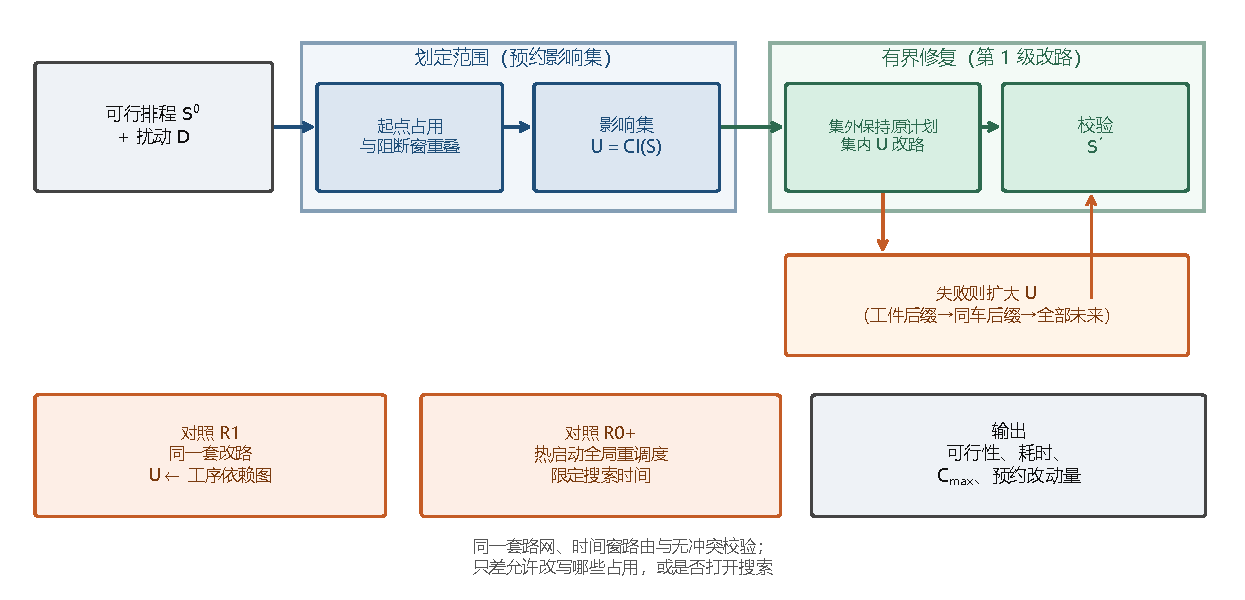
\includegraphics[width=\linewidth]{figures/fig_strc_framework_CN}
\caption{按预约影响集划界的有界恢复。
上排:由起点占用得到影响集并改路;中排:失败后扩大允许改写的范围;
下排:按工序依赖图划界的对照与热启动全局重调度对照,以及输出指标。
本图只画方法层的三条路径;毫秒档内另有三条对照(第~\ref{sec:cheap}~节)。}
\Description{三排流程图。上排:扰动进入后由起点占用得到预约影响集,集内占用允许改写、
集外保持原计划,然后原车改路。中排:改路失败时按工件后缀、同车后缀、
全部尚未结束占用的顺序扩大允许改写的集合并重试。下排:两条对照,
一按工序依赖图上的影响域划定范围,一做热启动全局搜索;三条路径汇入同一组输出指标。}
\label{fig:framework}
\end{figure}

\subsection{允许改写、保持原计划与第 1 级改路}
\label{sec:level1}

给定允许改写的占用集合 \(U\),第 1 级改路保持原车辆指派与机器指派,按原扫描序重放。
改路按走廊腿切分:车在 \(t_{\mathrm{now}}\) 已走完的腿属历史,原样预提交,
改路只从它当时所在的节点接着走;粒度粗于腿即会改写历史(注~\ref{rem:e2b_history})。
算法~\ref{alg:replay} 写出这一原语;算法~\ref{alg:strc_repair} 在它外面套预约影响集,失败则扩大 \(U\)。

\begin{algorithm}[t]
\caption{第 1 级改路重放 \(\textsc{ReplayReroute}\)}
\label{alg:replay}
\begin{algorithmic}[1]
\Require 排程 \(\mathcal{S}^0=(x,\pi,y,R)\), 扰动 \(\mathcal{D}\), 允许改写集合 \(U\), 时刻 \(t_{\mathrm{now}}\)
\Ensure 排程 \(\mathcal{S}'\) 或失败
\State 将 \(\mathcal{D}\) 写入路由层
  \Comment{阻断:禁行窗;通行变慢:重叠段 \(\tau\)}
\State 取空表 \(R'\)
\For{每条不可改写的占用:集外的全部,以及 \(r\in U\) 而 \(r.t^e\le t_{\mathrm{now}}\) 的}
  \State 将原字段 \((e,[t^s,t^e),k)\) 预提交到 \(R'\)
    \Comment{第二类是 A2 的历史,漏掉即等于改写历史}
  \If{与阻断窗冲突}
    \State \Return 失败
      \Comment{起点占用未覆盖与窗重叠的占用}
  \EndIf
\EndFor
\For{每条 \(r\in U\),按原扫描序}
  \State 从该车在 \(t_{\mathrm{now}}\) 的节点接起 \Comment{已走完的腿上一步已占位,不重复提交}
  \State 在当前 \(R'\) 上调用时间窗路由,提交新占用
    \Comment{不改写已经结束的占用}
\EndFor
\State 按 \(\pi\) 推进各机器空闲时刻与各工件就绪时刻
\State 独立校验:无冲突、无禁行窗残留、通行变慢的重叠段时长已吸收、集外字段未改
\If{校验通过}
  \State \Return \(\mathcal{S}'=(x,\pi,y,R')\)
\Else
  \State \Return 失败
\EndIf
\end{algorithmic}
\end{algorithm}

划界那一遍广度优先(定义~\ref{def:strc})只占耗时的一小部分:一次
\(\textsc{ReplayReroute}\) 还要对 \(|U|\) 个运输段各调用一次时间窗最短路,
实测耗时由后者主导(第~\ref{sec:e3}、\ref{sec:cheap}~节)。
该级不打开种群搜索。第~\ref{sec:e3}~节的对照固定算法~\ref{alg:replay},只替换 \(U\) 来自工序依赖图或预约影响集,
用以把可行率之差归因于划界对象。

\subsection{失败后扩大允许改写的范围}
\label{sec:scope_escalation}

扩大允许改写的范围,本身已有成例。Local Rescheduling~\cite{kuster2007local}
按时间窗逐步放宽直至可行;AOR 则按工件后继与同机后继纳入后续工序
(第~\ref{sec:rw_aor}~节)。本文沿预约依赖边扩大 \(U\),而不是沿时间窗。
这些步骤用来落实影响集:改路失败时仍先扩大须改写的占用,而不是立刻改开全局搜索。
第~\ref{sec:protocol}~节说明边界消融实验为何必须关闭这一步。

当集外占用保持过紧时,算法~\ref{alg:replay} 可能因运输--工序衔接等校验失败。
此时按下列顺序扩大 \(U\) 并重试同一套改路程序:
(i)~\(U\leftarrow U\cup\{\)当前 \(U\) 内各工序的同工件后缀、尚未结束的占用\(\}\);
(ii)~\(U\leftarrow U\cup\{\)所涉车辆的同车后缀、尚未结束的占用\(\}\);
(iii)~\(U\leftarrow\{\,r\in R:\ r.t^e>t_{\mathrm{now}}\,\}\)(把决策时刻尚未结束的占用全部纳入改写)。
扩大范围后仍是确定性的单遍改路。实验表明这一步可将可行率拉至全样本,算法耗时仍保持在毫秒至十余
毫秒量级(第~\ref{sec:experiments}~节)。这一步使耗时不随扰动比例 \(\varphi\) 单调变化,
因为两种效应方向相反:比例小时初始影响集偏紧、更常需要扩大范围,比例大时初始 \(U\) 已较松、
往往一轮成功,但单轮要改路的运输更多(读数见第~\ref{sec:scale}~节)。

\subsection{与全局重调度的对照}
\label{sec:vs_r0}

全局重调度对照在相同禁行约束下、在限定时间内以原排程为起点重新搜索(记 R0+)。
内部把 \((x,\pi)\) 编成一条染色体;一次\emph{解码}指:按该染色体的指派与扫描序,
在装了禁行窗的预约表上从头为全部运输调用第~\ref{sec:reservation}~节的时间窗路由,
得到新的 \(R\) 与 \(C_{\max}\)。R0+ 重复解码并允许改染色体;第~\ref{sec:cheap}~节的
RD 只解码一次且不改染色体。R0+ 的解码不改写已经结束的占用:这些占用预提交,
只从 \(t_{\mathrm{now}}\) 接着排未开始的工序(第~\ref{sec:e5}~节)。
对照取热启动而非从零搜索,以免丢掉原排程已有的指派与路径信息。
R0+ 可改派与改序,因而更可能缩短 \(C_{\max}\),但算法耗时由预算决定。

有界修复在完工时间上并不优于 R0+。第~\ref{sec:e5}~节表明:R0+ 在最小预算档上已占优,
而 R2 是定点、R0+ 随预算单调不增,故加预算也不出现反超。
有界修复的长处是算法耗时:响应须在毫秒量级时,它能恢复可行;允许秒级停机时,应用 R0+ 去缩短 \(C_{\max}\)。
集外占用的走廊、时段与车辆保持原计划,只在命题~\ref{prop:outside} 的条件下保证,实验中作部分观测。

只与 R0+ 对照会留下一个问题:毫秒量级那一档里,是否根本不需要按影响集划界?
把「不按影响集限制范围」的做法直接实现出来即可回答,本文取三种:全局右移(RS)不判断哪些占用
受影响,只把未完成占用整体后推到阻断结束之后;原染色体重解码(RD)不改染色体,只走一遍固定前缀解码;
\textbf{RA} 把 \(t_{\mathrm{now}}\) 之后尚未结束的占用全部纳入改写,再走与第~\ref{sec:level1}~节
\emph{完全相同}的改路程序,因而与本文方法只差「允许改写哪些占用」这一项——它是唯一能把预约影响集
单独隔离出来的对照。三者都在毫秒量级,构成有界修复在\emph{同一耗时档位内}的对照,
定义与读数见第~\ref{sec:cheap}~节。

算法~\ref{alg:strc_repair} 把本节与上节合起来写出,与图~\ref{fig:framework} 对应。

\begin{algorithm}[t]
\caption{基于预约影响集的有界恢复(第 1 级改路 + 扩大范围)}
\label{alg:strc_repair}
\begin{algorithmic}[1]
\Require 排程 \(\mathcal{S}^0\), 扰动 \(\mathcal{D}\), 时刻 \(t_{\mathrm{now}}\)
\Ensure 排程 \(\mathcal{S}'\) 或失败
\State \(S \gets \mathrm{Seeds}(\mathcal{D})\);
      \(U \gets \mathrm{Cl}(S)\)
\For{轮次 \(=0,1,2,3\)}
  \State \(\mathcal{S}' \gets \textsc{ReplayReroute}(\mathcal{S}^0,\mathcal{D},U,t_{\mathrm{now}})\)
  \If{\(\mathcal{S}'\) 可行}
    \State \Return \(\mathcal{S}'\)
  \EndIf
  \State 按扩大范围的规则更新 \(U\) \Comment{工件后缀 / 同车 / 全部尚未结束}
\EndFor
\State \Return 失败
\end{algorithmic}
\end{algorithm}

%% =====================================================================
\section{实验}
\label{sec:experiments}
%% =====================================================================

\subsection{协议}
\label{sec:protocol}

\textbf{路网、路由与算例.}
下层路网、时间窗路由与独立校验器固定。扩样矩阵使用\textbf{五个算例}:
小例 \texttt{example\_3x3x2}、拥堵例 \texttt{congested\_8x4x4},
以及三个 \texttt{S8x4x4} 布局 \texttt{high}、\texttt{funnel} 与 \texttt{mid}。
后三者同规模、同柔性,只差走廊拓扑,因此它们之间预约影响集规模的差异可归因于拓扑而非问题尺寸。
五者分两种来源:前两个是手写布局(小例供逐步核对,拥堵例为哑铃拓扑);后三个由本文的算例
生成器产生,其参数——工件数 \(\times\) 机器数 \(\times\) AGV 数、拥堵档、\(H\)、\(F\)——
与\textbf{生成随机种子}一并编码在算例文件名中,三者的生成种子同为 \(42\)。
\textbf{生成随机种子与下文的运行随机种子是两回事}:前者只决定算例本身,后者决定扰动注入
与搜索过程;两者在取值上都出现 \(42\) 纯属巧合,不存在共用。
\textbf{随机种子取十个},即 \(42\)、\(7\)、\(2024\)、\(99\)、\(123\)、\(13\)、\(1\)、
\(777\)、\(31415\) 与 \(8\),共 \(\NInst\times\NSeeds=\NPairs\) 个算例--随机种子对。
全文所有逐格比较、胜负计数与配对检验都按 (算例, 随机种子) 这一对键对齐:
同一键下各方法读取同一份初始解、同一段阻断与同一决策时刻。
初始排程由第~\ref{sec:reservation}~节的时间窗路由按扫描序重放得到,
并通过独立无冲突校验;同一算例--随机种子对下各对照方法共享该初始解。
本文不依赖这份 \(\mathcal{S}^0\) 的搜索来源,只要求它在扰动前可行。

\textbf{实现与运行环境.}
全部实验为纯 Python 标准库实现,不依赖第三方数值库;下层路网、时间窗路由与独立校验器
复用与静态一体化工作同一份实现。单机单线程运行,不使用并行:Intel Xeon W-1270
(\(8\) 核 \(16\) 线程)、\(64\)\,GB 内存、Windows 10,解释器为 CPython \(3.7.6\)(\(64\) 位)。
因不引入第三方数值库,复现不需要锁定依赖版本;\(3.7\) 是本文实测的解释器,
更高版本未逐一复跑。所有计时读数都在上述单机单线程条件下取得,
换机器会整体平移,故本文一切耗时结论都以\emph{比值}或\emph{量级}形式给出,不用绝对毫秒立论。

\textbf{代码与数据可用性.}
复现所需材料分三部分:上层有界修复与实验驱动、下层路网与时间窗路由、
算例与扰动输入及全部逐格读数(CSV)。三者连同重跑各表各图的脚本一并提交,
审稿期间以\textbf{匿名仓库}形式提供(见投稿系统所附链接,仓库内不含作者身份信息);
论文接受后转为公开仓库并在永久存档服务上登记 DOI,本节届时补填该 DOI。
每张表与每幅图在仓库中都能追到生成它的脚本与对应的 CSV,
表~\ref{tab:instscale} 所列算例亦随仓库分发。

\textbf{第二批:布局出处外部化.}
上面五个算例的布局都是本文设计的,其中三张同规模布局还同属哑铃一族(彼此只差装卸点
出口与中段的并行通道数,即只差容量、不差几何)。为了让布局不再由本文决定,另跑一批
\NPubInst\ 个算例:路网的网格尺寸、装卸站与机器落位、断掉的边这三项逐项转录自
Lyu 等~\cite{lyu2019approach} 附录 A 的布局图,转录结果由脚本与 van Os 配套工具集
所给的机读编码逐字段对账。机器台数因此由布局决定而非由本文选定,为 \(4\) 至 \(8\) 台。
随机种子仍取同样十个,合计 \NPubPairs\ 个算例--随机种子对。两批算例\emph{逐参数同口径}:工件数、
AGV 数、每工件工序数、\(H\)、\(F\) 以及运输/加工时长比的标定目标一律相同,于是两批之差
可以干净地归因给布局出处。

该附录共给出六张布局(\(3\) 至 \(8\) 机)。\(3\) 机那张未用:固定 \(F=0.6\) 在 \(|M|=3\) 时
给出平均候选机数 \(1.8<2\),与「每道工序至少两台候选机」不相容,而为一张布局放宽 \(F\)
会多引入一个变量。

其余五张\textbf{只落在 \NPubNets\ 张不同路网上},须先说明:\(4\) 机与 \(5\) 机两张共用
同一张 \(4\times 4\) 网格(去掉同一条边),\(6\)、\(7\)、\(8\) 机三张共用同一张
\(5\times 5\) 网格(去掉同两条边);五者彼此的差别在于机器台数与\emph{落位},
而非路网几何。这是原始发布件本身的组织方式,不是本文的取舍。因此第~\ref{sec:e4}~节读这批
数时,\textbf{路网几何这一维的独立样本是 \NPubNets\ 而不是 \NPubInst},而机器落位这一维
有 \NPubInst\ 个;下文的论断严格按这个划分来下。

有三处口径必须先声明清楚。\textbf{其一,逐段行驶时间不是原始数据。} Lyu 只为单个示例
算例发表过逐段时长,且其取值并不均匀;附录 A 那批布局的逐段时长从未发表。故这里按
"所有边等权"补齐——它与 van Os 模型里"单步时长为常量"的假设在结构上一致,只是时间单位的
标度不同。\textbf{因此本批结果不可与 Lyu 或 van Os 的参照值作任何比较};它提供的只是
一批不由本文设计的拓扑,而不是一个对标集。\textbf{其二,装卸点做了合并。} 原布局有分离
的装货站与卸货站,本文只有一个装卸点,故取车辆起始处的装货站充当该点,卸货站退化为普通
网格节点。\textbf{其三,工件数据没有一并借用。} 已实测的公开族里平均运输时长只占平均
加工时长的百分之几,运输在其上几乎不构成争用;若把工件数据也搬进来,走廊争用连同以它
为对象的整套结论都会退化到观察不到。外部化的只有路网。
同一工具集另附的一族布局(其目录标注为 Liu 2023)未纳入本批:这些布局的数据声明允许对角
移动,而本文的走廊是四邻接的;接受对角移动要改的是下层路由而不是算例。

\textbf{扰动.}
除非另注,\(t_{\mathrm{now}}=0.35\,C_{\max}(\mathcal{S}^0)\)。
E1--E3/E5 在繁忙走廊上施加单窗阻断;E6 在同一 \(t_{\mathrm{now}}\) 上另加三类扰动;
规模扫描将未来工序按最早未来预约排序,取前比例 \(\varphi\) 的预约时窗作为微阻断(不合并)。

\textbf{对照方法.}
R1:按工序依赖图上的影响域划界 + 第 1 级改路,全文取 \(\theta=2\)
(该值只影响 A 类扰动下 \(|U_{R1}|\) 的大小;由命题~\ref{prop:miss},B 类上
任何有限 \(\theta\) 都给出空集);其划界规则取自第~\ref{sec:rw_aor}~节所述的工序级
局部重调度做法,由本文重新实现。逐条对应关系是:「受影响工序集取直接受扰工序,
再沿工件内工序先后关系向后扩张」这一条划界规则对应
AOR~\cite{abumaizar1997rescheduling,subramaniam2003maor};
而\emph{以跳数 \(\theta\) 截断扩张}、以及\emph{把工序集映射为须释放的走廊预约}
两项由本文写定——原文的设定里没有预约表,这一映射在原文中无对应物;
改路与重放部件则与 R2 共用同一份实现,以保证两者只差划界对象。
因此 R1 是「把该划界规则移到本文预约设定下」所得的对照,\textbf{不是对上述文献的复现};
第~\ref{sec:e3}~节它的读数只说明该划界规则在此设定下给出空范围,
不构成对原方法在其自身设定下的评价;
R2/\STRC:按预约影响集划界 + 第 1 级改路(规模扫描打开失败后扩大范围;E3/E5 关闭这一步);
R0+:以原排程为起点、在限定时间内重新搜索的全局重调度——遗传算法,种群 \(40\),
原排程对应的染色体置入初始种群,解码走与 RD 同一套固定前缀解码(\(t_{\mathrm{now}}\)
之前的占用不可改写);\emph{不设代数上限与早停阈值},终止条件只有挂钟预算一项,
预算取值见第~\ref{sec:e5}~节;
RS:全局右移,不按影响集划界且不改路(第~\ref{sec:cheap}~节);
RD:原染色体重解码,即本实现里耗时更短的一次全局重算(同节);
RA:不按影响集限制范围、但保留改路——把 \(t_{\mathrm{now}}\) 之后尚未结束的占用全部纳入改写,其余与 R2 逐项相同,
用于把预约影响集这一项单独隔离出来(同节)。
这五条对照按「是否划界 \(\times\) 重算多少」铺开:R1 与 R2 只差划界\emph{对象},
RA 与 R2 只差\emph{是否}划界(改路程序完全相同),RS 既不划界又放弃改路而整体后推,
RD 与 R0+ 则重算全局而不按影响集划界,只差搜索多少代。

\textbf{预算口径.}
各法不在同一预算档上比较,这一点须先说明:R1、R2、RS、RD、RA 均为一次确定性修复,
跑完即止,耗时由算例规模与影响集大小决定而非由预算设定;只有 R0+ 按挂钟预算终止。
因此 R0+ 与其余各法之间不存在同挂钟、同代数或同评价次数的对齐,凡涉及 R0+ 的读数
一律按「给定预算下的读数」理解;第~\ref{sec:cheap}~节的四法对照才是同一预算档内
(均跑完即止)的比较。挂钟耗时按批次报告,不跨批次并读。

\textbf{一处必须写清的口径.}
E3 中\emph{必须关闭}失败后扩大范围。若开着,R1 会靠「一路扩到把尚未结束的占用全部纳入改写」而偶然成功,
测到的就不再是划界对象的差别,而是扩大规则的兜底能力。扩大范围本身有效(规模扫描中它把可行率
拉满),但它与被测变量正交,故在边界消融中一律关闭。
该端点并未因此被回避:它就是第~\ref{sec:cheap}~节的 RA,那里作为独立对照逐格测了
它的代价。

\textbf{两批算例各自承担什么.}
两批不是同一组证据的两次采样,它们回答的问题不同,故本章各节只由其中一批支撑。
主批次回答\emph{现象是否存在、机制是否干净}:B 类扰动下按工序依赖图划界得到空范围而原排程不可行
(第~\ref{sec:e1}~节)、预约影响集对该范围的包含与集外字段的不变性(第~\ref{sec:e2}~节)、
同一套改路程序下只替换划界对象的对照(第~\ref{sec:e3}~节)。这三件事都要求对算例参数有完全的
控制权,尤其是运输/加工时长比——它决定走廊争用是否成立——而公开族给不了这种控制权
(第~\ref{sec:limitations}~节局限第 4 条)。第二批回答的是另一个问题:\emph{这些现象
是否只在本文自选的布局上成立}。它因此只用于复现,不产生新的性能读数
(第~\ref{sec:pubrepro}~节)。

两处需要点明。其一,\textbf{第二批用来检验现象是否只在本文自选布局上成立},
并收窄结构可预测性的结论(第~\ref{sec:e4}~节)。
其二,\textbf{只有 E4 一格必须两批合读}:主批次的三张同规模布局同属一族、只差容量不差
几何,在它们身上"指标太粗"与"算例集几何差异不足"这两种解释混在一起;而外部布局若没有
逐参数同口径的自建对照,也无从判断其影响集占比的变动幅度算不算大。其余各节的结论由主批次
单独成立,第二批只增强其外部效度。

\textbf{统计口径.}
全文只有一处推断性检验:第~\ref{sec:cheap}~节 R2 与 RA 在改动比例上的差,
采用 Wilcoxon 符号秩检验,双侧,按上述 (算例, 随机种子) 键配对。
因为全文只做这一次检验,不构成多重比较,故未做校正;其余各处的逐格胜负、均值与中位
一律是\emph{描述性}统计,不作显著性断言。
该检验配套的效应量报为 Hodges--Lehmann 估计 \(0.037\),\(95\%\) 自助置信区间
\([0.018,\,0.074]\)(百分位法,\(10^4\) 次重采样,固定随机种子);配对差的均值为
\(\RAStabMean\),区间 \([0.039,\,0.093]\)。离散度按四分位距报告:改动比例在 R2 上为
\(0.073\)、在 RA 上为 \(0.062\)。% selfcheck:allow-num 0.073 为 R2 改动比例的四分位距,与 \RAStabMeanNet(剔除恒等格后的平均降幅)同值不同源因 \(50\) 格中有 \(18\) 格两法恰好持平,配对差
\emph{中位}的区间下端触 \(0\)——这一点如实记下,它说明胜负计数里的持平格占了三分之一。
其余各批次的表格只给均值、中位与计数,不含区间。

\subsection{E1:工序依赖图给出空范围}
\label{sec:e1}

本节只问一件事:B 类扰动下两种划界各给出什么范围,不比较修复质量。
表~\ref{tab:e1} 与图~\ref{fig:e1e3}(左)按第~\ref{sec:protocol}~节的走廊阻断协议汇总命题~\ref{prop:miss} 的扩样结果:
\(\PassMiss\) 样本上 \(T_{\mathrm{impact}}=0\)、起点占用与预约影响集非空、阻断后原排程不可行,
结构泄漏均为 \(0\)。

按命题~\ref{prop:miss} 之后那段话的提醒,读这张表时重量应压在\emph{后半句}上。
\(T_{\mathrm{impact}}=0\) 这一列是定义~\ref{def:task_impact} 对 B 类约定的推论,
它把「工序依赖图按定义覆盖不到走廊阻断」显示出来,但本身不是发现。
非平凡的是\(\texttt{feasible\_after\_block}\) 一列恒为假——排程\emph{确实}已经不可行。
两者合起来才构成反例。

\begin{table}[t]
\centering
\caption{E1 走廊阻断下工序依赖图给出空范围(每算例 \(\NSeeds\) 个随机种子,共 \(\NPairs\) 对)。
\(|R|\) 为全表占用数,\(\mathrm{Cl}/|R|\) 为预约影响集占全表的比例。均值取多种子平均。
离散度按四分位距(IQR)报告:逐算例 \(\mathrm{Cl}/|R|\) 的 IQR 在
\EoneFracIqrLo--\EoneFracIqrHi 之间,\(\NPairs\) 对合池的中位为 \EoneFracMed、
极差 \EoneFracMin--\EoneFracMax;可见该比例的算例间差异与种子间差异同量级,
不宜只读均值。
「C1 通过」为命题~\ref{prop:miss} 三条件同时成立的格数(\(T_{\mathrm{impact}}=0\)、
起点占用非空、阻断后原排程不可行)。后三行同规模同柔性,只差走廊拓扑。}
\label{tab:e1}
\small
\begin{tabular}{@{}lcccccc@{}}
\toprule
算例 & 随机种子 & C1 通过 & 均 \(|R|\) & 均 \(|\mathrm{Seeds}|\)
 & 均 \(|\mathrm{Cl}|\) & \(\mathrm{Cl}/|R|\) \\
\midrule
\texttt{example\_3x3x2}   & 10 & \(10/10\) & \(28.6\)  & \(5.6\)  & \(16.9\) & \(0.59\) \\
\texttt{congested\_8x4x4} & 10 & \(10/10\) & \(85.0\)  & \(15.0\) & \(48.4\) & \(0.57\) \\
\texttt{S8x4x4} (high)    & 10 & \(10/10\) & \(150.5\) & \(15.5\) & \(88.3\) & \(0.59\) \\
\texttt{S8x4x4} (funnel)  & 10 & \(10/10\) & \(149.1\) & \(15.5\) & \(85.4\) & \(0.57\) \\
\texttt{S8x4x4} (mid)     & 10 & \(10/10\) & \(147.6\) & \(15.0\) & \(82.8\) & \(0.56\) \\
\midrule
合计 & \(\NPairs\) & \(\PassMiss\) & --- & --- & --- & --- \\
\bottomrule
\end{tabular}
\end{table}

\(|\mathrm{Cl}|\) 的绝对值随算例变大(\(16.9\)、\(48.4\)、\(82.8\)--\(88.3\)),这是占用总数变多的直接结果;
而 \(\mathrm{Cl}/|R|\) 在五个算例上都落在 \EoneCloLo--\EoneCloHi,\emph{未能}区分三个 \(\texttt{S8x4x4}\) 布局。
这与第~\ref{sec:e4}~节的结论一致:实验没有给出能可靠预测影响集规模的结构指标。
就贡献而言,本节只坐实一件事:B 类扰动下按工序依赖图划界得到空范围,而原排程确已不可行;
\(\mathrm{Cl}/|R|\) 的具体数值不承担任何主张。

\subsection{E2:包含性}
\label{sec:e2}

结构包含性(E2a)在 \(\PassClosed\) 样本上成立(泄漏 \(=0\)),与命题~\ref{prop:struct} 一致。
第 1 级修复(不扩大范围)在 \(\NPairs/\NPairs\) 样本上可行。
集外占用的走廊、时段与车辆逐条不变(E2b / 命题~\ref{prop:outside} 的观测形式)同样在 \(\PassInvar\) 样本上
成立(表~\ref{tab:e2})。

\begin{table}[t]
\centering
\caption{E2 包含性(\(\NSeeds\) 个随机种子/算例;第 1 级可行一列不扩大范围)。
E2a 为结构闭合(泄漏 \(=0\)),
E2b 为集外占用的走廊、时段与车辆\emph{逐条}不变。}
\label{tab:e2}
\small
\begin{tabular}{@{}lccc@{}}
\toprule
算例 & E2a 闭合 & 第 1 级可行 & E2b 集外逐条不变 \\
\midrule
\texttt{example\_3x3x2}   & \(10/10\) & \(10/10\) & \(10/10\) \\
\texttt{congested\_8x4x4} & \(10/10\) & \(10/10\) & \(10/10\) \\
\texttt{S8x4x4} (high)    & \(10/10\) & \(10/10\) & \(10/10\) \\
\texttt{S8x4x4} (funnel)  & \(10/10\) & \(10/10\) & \(10/10\) \\
\texttt{S8x4x4} (mid)     & \(10/10\) & \(10/10\) & \(10/10\) \\
\midrule
合计 & \(\PassClosed\) & \(\NPairs/\NPairs\) & \(\PassInvar\) \\
\bottomrule
\end{tabular}
\end{table}

需要区分 E2a 与 E2b 说的不是一回事,\emph{满通过并不使命题~\ref{prop:outside}
升格为充要}。E2a 是\emph{图上的}性质,由命题~\ref{prop:struct} 保证,满通过是应当的;
若不满通过,说明实现与定义不符。E2b 是\emph{修复之后的}性质,它检验的是命题的四条前提
在本文协议下是否成立——而不是这些前提可以省略。特别地,前提 (ii) 要求集外占用逐条
预提交成功;若某条集外占用与禁行窗重叠,预提交即失败,那说明起点占用集不完备
(注~\ref{rem:precommit}),此时命题不适用。本文的实验落在前提成立的一侧,
不等于任何设定下都会落在那一侧。
收口到贡献:E1、E2 与第~\ref{sec:e3}~节的边界消融支撑的是\emph{对象成立}这一层——预约影响集
由边集唯一确定、对外封闭,且在同一套改路程序下足以恢复可行;按这个对象划界比不划界
多出多少收益是\emph{另一层},只由第~\ref{sec:cheap}~节的 RA 对照支撑。

\begin{remark}[一处曾经把实现缺陷读成边集缺陷的教训]
\label{rem:e2b_history}
这一栏在早前的批次上只有 \(24/\NPairs\)。当时的解读是「依赖边集未能覆盖若干弱耦合」,
并据此把加细边集列为首要后续工作。复核后该解读是错的。允许改写的是一个\emph{占用}集合,
而重放时是否改路却按\emph{工序}判定——同一工序的空载段与满载段只要有一段落在影响集内,
整道运输就被重规划。于是当只有满载段进入影响集时,同工序的空载段也被改写,而它的任务
标签并不在允许改写的集合内,遂被记为集外漂移。\(26\) 个不通过格上的 \(84\) 条漂移占用无一例外
都是这种同工序空载段,其中 \(71\) 条(\(85\%\))在 \(t_{\mathrm{now}}\) 之前就已执行完毕
——改写它同时违反「不改写已经结束的占用」。改为按\emph{段}判定(已执行完或未纳入改写的空载段沿用原计划,
只改路真正落在允许改写集合内的段)之后,漂移归零。
换言之,此前测到的不是边集对物理耦合的覆盖度,而是命题~\ref{prop:outside} 前提 (iii)
「仅对 \(U\) 内运输调用路由器」在实现上没有被真正满足。记下这一条,是因为它示范了一种
容易发生的误判:把实现与定义的粒度错配,读成模型对世界的刻画不足。

\textbf{同一类错配还剩一层,而 E2b 查不到它。} 按段判定之后,一个\emph{跨越}
\(t_{\mathrm{now}}\) 的运输段仍是整段重规划:只要它有一条走廊腿的结束时刻落在
\(t_{\mathrm{now}}\) 之后,整个段的任务标签就进入允许改写的集合,于是它在 \(t_{\mathrm{now}}\)
之前\emph{已经走完}的那几条腿也被重排——等于把车退回该段起点重走一遍,违反「不改写已经结束的占用」。
E2b 查不出这一情形,因为这些腿的任务标签在影响集\emph{内},本就不在集外字段的比对范围里。
用一项独立的「已结束占用不可改写」审计(逐条比对 \(t_{\mathrm{end}}\le t_{\mathrm{now}}\)
的占用)才测出来:\(\NPairs\) 个格子里有 \(36\) 个存在此类改写,合计 \(86\) 条。
把粒度再细一层——按\emph{走廊腿}切分,已走完的腿原样保留,改路只从车在
\(t_{\mathrm{now}}\) 时实际所处的节点往后接——之后该审计在全部 \(\NPairs\) 个格子上归零,
且各项通过率不变、\(C_{\max}\) 在 \(6\) 个格子上变好、无一格变差。
本文报告的是修正后的读数。本注的历史读数(\(24/\NPairs\)、\(26\) 格 \(84\) 条、\(36\) 格 \(86\) 条)
来自修正前的批次与一次独立的「已结束占用不可改写」审计,不在本文任何表中,也不参与任何主张。
\end{remark}

\subsection{E3:边界消融}
\label{sec:e3}

表~\ref{tab:e3} 与图~\ref{fig:e1e3}(右)固定第 1 级改路并\emph{关闭}失败后扩大范围。
B 类上 \(\NPairs/\NPairs\) 样本 R1 的允许改写集合为空且不可行,R2 全部可行。

这是本文最强的一组对照,但它的说服力来自\emph{只差一项}而不是来自数字大:
同一套改路程序、同一份初始解、同一个 \(t_{\mathrm{now}}\)、同一批随机种子、同一段阻断窗,
\textbf{唯一的差别是允许改写哪些占用}。因此 \(\FeasRone\) 对 \(\FeasRtwo\) 这个反差不能
归因于改路启发式的优劣——R1 侧根本没有触发任何改路,它的允许改写集合是空的,
第 1 级改路对空集是恒等操作,于是原排程原封不动地留在被阻断的走廊上。
换句话说,R1 的失败方式不是「修得不好」,而是「判断为无需修」。
第 1 级改路逐格的耗时中位数为 \(\MsRepairMed\)\,ms、最大 \(\MsRepairMax\)\,ms;表~\ref{tab:e3} 末列
是各算例内 \(\NSeeds\) 个种子的均值,两者口径不同,不可对读。
就贡献而言,本节把缺口的成因定在划界对象上:同一套改路程序只换划界对象,恢复可行率即从
\(\FeasRone\) 变到 \(\FeasRtwo\);这仍属\emph{对象成立}那一层,不涉及划界值不值。

\begin{table}[t]
\centering
\caption{E3 边界消融(不扩大范围;\(\NInst\) 算例 \(\times\) \(\NSeeds\) 个随机种子)。
miss\_B 指该格上 R1 的允许改写集合为空而 R2 非空。
末列为各算例内 \(\NSeeds\) 个种子的均值,与正文逐格中位数口径不同。}
\label{tab:e3}
\small
\begin{tabular}{@{}lccccc@{}}
\toprule
算例 & miss\_B & R1 可行 & R2 可行 & 均 \(|U_{R2}|\) & R2 耗时/ms \\
\midrule
\texttt{example\_3x3x2}   & \(10/10\) & \(0/10\) & \(10/10\) & \(16.9\) & \(0.66\) \\
\texttt{congested\_8x4x4} & \(10/10\) & \(0/10\) & \(10/10\) & \(48.4\) & \(2.84\) \\
\texttt{S8x4x4} (high)    & \(10/10\) & \(0/10\) & \(10/10\) & \(88.3\) & \(3.40\) \\
\texttt{S8x4x4} (funnel)  & \(10/10\) & \(0/10\) & \(10/10\) & \(85.4\) & \(5.09\) \\
\texttt{S8x4x4} (mid)     & \(10/10\) & \(0/10\) & \(10/10\) & \(82.8\) & \(3.96\) \\
\midrule
合计 & \(\NPairs/\NPairs\) & \(\FeasRone\) & \(\FeasRtwo\) & --- & --- \\
\bottomrule
\end{tabular}
\end{table}

\begin{figure}[t]
\centering
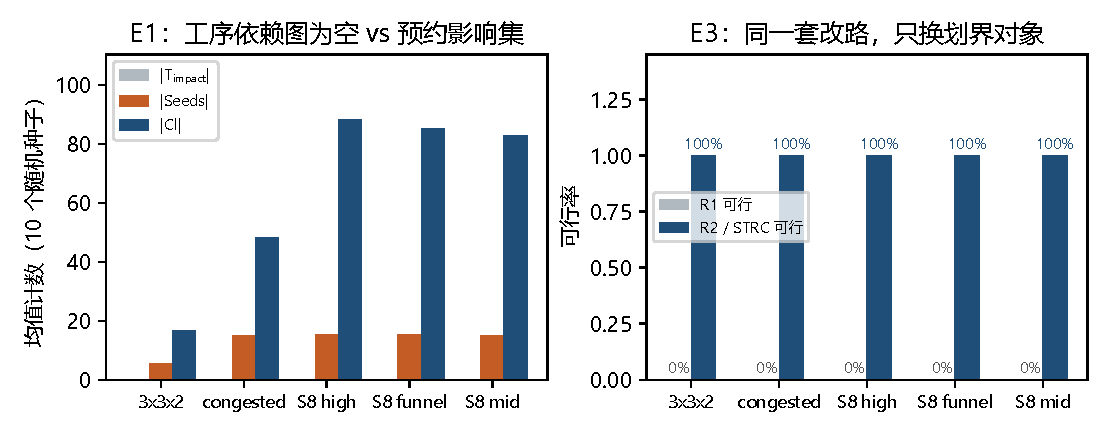
\includegraphics[width=\linewidth]{figures/fig_strc_e1e3_CN}
\caption{E1/E3 扩样可视化(\(\NInst\) 算例 \(\times\) \(\NSeeds\) 个随机种子均值)。
左:工序依赖图上的影响域为空,而起点占用与预约影响集非空;柱高为每算例 \(\NSeeds\) 格
的均值,离散度按四分位距见表~\ref{tab:e1}(\(|\mathrm{Cl}|\) 的 IQR 逐算例在 \(2\)--\(8\)
之间,影响域一组恒为零故无离散度)。
右:同一套改路、只换划界对象时 R1 可行率为 \(0\)、R2 为 \(100\%\);该幅为逐格计数
(各 \(\NPairs\) 格),不是均值,故不配离散度。}
\Description{并排两幅条形图。左幅按五个算例给出工序依赖图影响域、起点占用数与预约影响集规模
三组柱子,影响域一组恒为零,另两组随算例规模上升。右幅给出两种划界的恢复
可行率,按工序依赖图划界一侧为零,按预约影响集划界一侧为百分之百。}
\label{fig:e1e3}
\end{figure}

%% 标题里不放 \(\times\):它会进 PDF 书签,hyperref 无法处理数学模式。
\subsection{E6:扰动类型与边界定义的交叉}
\label{sec:e6}

E1--E3 只用了走廊阻断一种扰动。本小节把扰动类型这一维展开,在同一 \(\NPairs\) 对上另加
走廊通行变慢、车辆故障与机械臂故障三类,给出表~\ref{tab:e6}。

\textbf{先说测什么。} 划界一侧四类都报:工序依赖图上的影响域有多大、预约影响集有多大、后者是否包含前者。
修复一侧四类都开口。B 类仍只改路:阻断把禁行窗写入预约表,通行变慢在窗内按倍率
\(\tau_{\mathrm{mult}}=2\) 降低进度、窗外仍走原 \(\tau\),走廊仍可走。
A 类额外换车或改派,不改扫描序;是否扩大允许改写的范围,对它们不改变动作集合。

\begin{table}[t]
\centering
\caption{E6 扰动类型 \(\times\) 划界对象(\(\NPairs\) 对/类,共 \(200\) 次测量;
其中两类 B 扰动按构造给出同一起点集,故\emph{独立}划界测量为 \(150\) 次,见正文第三点)。
\(|R^{\circ}|\) 为 \(t_{\mathrm{now}}\) 之后尚未结束的占用数。
「R1 为空」即按工序依赖图划界判该扰动无需重调度的格数。
末列不扩大范围:B 类为第 1 级改路,A 类为换车或改派。}
\label{tab:e6}
\small
\begin{tabular}{@{}llccccc@{}}
\toprule
扰动 & 类 & R1 为空 & 均 \(|U_{R1}|\) & 均 \(|\mathrm{Cl}|\)
 & \(\mathrm{Cl}/|R^{\circ}|\) & R2 可行 \\
\midrule
走廊阻断   & B & \(50/50\) & \(0.0\)  & \(64.4\) & \(0.92\) & \FeasESixBlock \\
走廊通行变慢 & B & \(50/50\) & \(0.0\)  & \(64.4\) & \(0.92\) & \FeasSlow \\
车辆故障   & A & \(0/50\)  & \(31.1\) & \(60.6\) & \(0.85\) & \FeasESixAgv \\
机械臂故障 & A & \(0/50\)  & \(42.8\) & \(65.9\) & \(0.94\) & \FeasESixRa \\
\bottomrule
\end{tabular}
\end{table}

四点读数。第一,\textbf{A/B 二分在 \(150\) 次\emph{独立}划界测量上无一例外}(两类 B 扰动按构造
共用同一起点集,见下面第三点,故不计作 \(200\) 次):两类 B 扰动按工序依赖图划界
全部为空,两类 A 扰动全部非空。第二,\textbf{在全部 \(100\) 次 A 类测量上
\(U_{R1}\subseteq\mathrm{Cl}\)}——这说明改用预约影响集划界在 A 类上不会\emph{丢掉}
工序依赖图已纳入的占用。包含在 \(\StrictlyLarger\) 上是严格的,其余 \(13\) 格两者恰好相等
(此时影响集沿依赖边没有走出工序依赖图影响域诱导的那个集合),\emph{不是}包含失败。
其中机械臂故障那 \(50\) 格的包含\emph{按构造}成立:定义~\ref{def:seeds}(c) 的起点规则沿工件链
取整条后缀,而 \(U_{R1}\) 以 \(\theta=2\) 截断(第~\ref{sec:protocol}~节),
故该行验证的是实现与定义一致,不是一项独立发现;车辆故障那 \(50\) 格的包含不由构造给出,
是实测结果。
代价是允许改写的集合平均变大:车辆故障 \(31.1\to 60.6\),机械臂故障 \(42.8\to 65.9\)。
结合第一点,预约影响集在这四类扰动上对工序依赖图划界是\emph{覆盖面}的一致加强——不丢任何
已纳入的占用;但它在集合规模上确有代价,两者不是覆盖面上的此消彼长。
第三,\textbf{通行变慢与阻断的划界两行逐格相同},在全部 \(50\) 对上影响集规模一致。
这不是两次独立的划界验证:起点规则对二者都是「与失效时窗重叠、尚未结束的占用」,
故它们按构造给出同一个起点集,进而给出同一个预约影响集。该行证实的是按工序依赖图划界对通行变慢同样为空。
第四,\textbf{修复一侧四类均满},逐类读数见表~\ref{tab:e6} 末列,通行变慢与阻断同口径。
通行变慢一度把与窗有交的穿越整段乘 \(2\),\(13\) 格死在「占用偏短」——
窗内 \(2\tau\) 无空档时,进入时刻被拉回窗内却仍按原 \(\tau\) 落盘;
其中 \(12\) 格连把尚未结束的占用全部纳入改写也过不了,故不是集外保持原计划把变慢的车卡死。
改为只缩放重叠进度之后,第 1 级满通过,不再触发扩大范围。
走廊仍可走,与「整段封死再绕路」的物理差别还在,只是不再被整段倍率放大。
车辆故障走换车,机械臂故障走改派。
换车与改派是落实 A 类恢复的动作,用来补全覆盖矩阵的修复一侧。

\textbf{这张表也给出了影响集规模的实测}(注~\ref{rem:minimality})。
走廊阻断下预约影响集覆盖 \(t_{\mathrm{now}}\) 之后尚未结束占用的约 \(\ClosureAliveFrac\);
相对「把尚未结束的占用全部纳入改写」这一平凡上界只少纳入不足一成。有界修复真正省下的是不改写已经结束的占用与不重开搜索,
而不是把未来切得很小。第~\ref{sec:e1}~节按全表统计的 \(\mathrm{Cl}/|R|\) 落在 \EoneCloLo--\EoneCloHi
与此不矛盾:全表包含 \(t_{\mathrm{now}}\) 之前已经执行完毕、本就不可改的那一半。
两个口径都给出。就贡献而言,本节只扩了\emph{覆盖面}——把 A/B 二分与包含性从一种扰动推到四种;
它没有加强任何一条主张的强度,也没有引入新的划界对象。

\subsection{案例甘特}
\label{sec:case}

\begin{sloppypar}
E1--E3 给出的是跨随机种子的计数与可行率。为把「工序依赖图覆盖不到、预约影响集可修」落到时间轴上,
图~\ref{fig:case} 取 \texttt{example\_3x3x2}、随机种子 \(42\) 的一例走廊阻断,
协议同 E2/E3:决策时刻取 \(0.35\,C_{\max}\),繁忙走廊单窗阻断,第 1 级改路、不扩大范围。
\end{sloppypar}

该例上 \(T_{\mathrm{impact}}=\varnothing\),而 \(|\mathrm{Seeds}|=6\)、\(|\mathrm{Cl}|=18\)。
图~\ref{fig:case}(a) 为扰动前原排程的机器甘特:蓝色工序的运输占用落入影响集(将被改路),
灰色工序在影响集外(预提交、保持原计划);红色虚线为 \(t_{\mathrm{now}}\),浅红带为阻断时窗。
图~\ref{fig:case}(b) 为修复后:影响集内工序时间轴重排,排程在阻断下恢复可行,
\(C_{\max}:57\to 86\),耗时亚毫秒级。
本图只说明统计结论对应何种局部改动形态,不用于比较完工时间;
完工时间与全局重调度的权衡见随后的 E5 与规模扫描。

\begin{figure}[t]
\centering
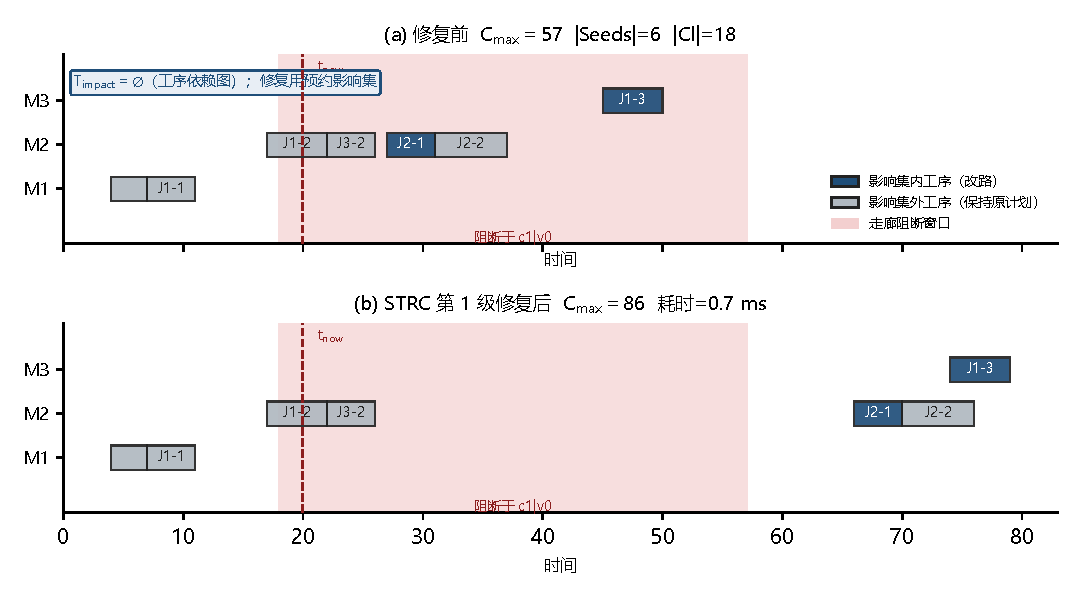
\includegraphics[width=\linewidth]{figures/fig_strc_case_CN}
\caption{案例甘特(\texttt{example\_3x3x2}, 随机种子 \(42\))。
(a)~阻断前原排程,按是否属于 \(\mathrm{Cl}\) 着色;
(b)~第 1 级修复后。工序依赖图上的影响域为空;蓝色工序对应影响集内运输被改路。
本图为\emph{存在性}演示:说明统计结论对应何种局部改动形态,\(C_{\max}\) 的变化不作性能读数。}
\Description{上下两幅机器甘特图。(a) 阻断前的原排程,条块按其运输占用是否落在
预约影响集内着蓝灰两色,一条竖直红虚线标出决策时刻,一条浅红竖带标出阻断时窗。
(b) 修复后的排程,蓝色条块的时间轴被重排,灰色条块位置不变,完工时间由 57 增至 86。}
\label{fig:case}
\end{figure}

\subsection{E4:结构(探索)}
\label{sec:e4}

在 LU 割边阻断下,funnel 与 high 的预约影响集占比随随机种子波动(表~\ref{tab:e4})。
方向上确实是 funnel 更高——中位 \(0.254\) 对 \(0.204\),均值 \(0.244\) 对 \(0.229\)
——但\emph{两组取值高度重叠}:funnel 落在 \([0.180,0.309]\),high 落在
\([0.156,0.372]\),后者的区间把前者整个包住,且单个随机种子即可反向
(\(2024\) 一列上 high 的 \(0.372\) 反高于 funnel 的 \(0.296\))。
五个随机种子、两个布局,这个差距不足以支撑任何结论。
第~\ref{sec:e1}~节按繁忙走廊阻断协议在三个同规模布局上得到的
\(\mathrm{Cl}/|R|\) 亦落在 \EoneCloLo--\EoneCloHi 的窄带内,同样未能区分布局。

\textbf{换一批不由本文设计的布局,这条负结果的成因才分得清.}
三张同规模布局同属哑铃一族,几何差异很小(见表~\ref{tab:e4pub}:节点数 \(9\)--\(11\)、
走廊数 \(8\)--\(12\),LU 割仅在 \(1\) 与 \(2\) 之间);"指标太粗"与
"算例集几何差异不足"这两种解释在它们身上混在一起,无从分辨。第~\ref{sec:protocol}~节的
第二批把两者分开(表~\ref{tab:e4pub})。

\textbf{结果的方向与预期相反,而这恰是关键.}
按第~\ref{sec:protocol}~节的声明,这批算例在路网几何上只有 \NPubNets\ 个独立样本,
故\emph{不能}用它来论证"影响集占比随路网几何变化";能论证的是另一件事。
在\emph{同一张} \(4\times 4\) 路网上,只把机器台数与落位从 \(4\) 机换成 \(5\) 机,
影响集占比中位即由 \PubCloHi\ 落到 \PubCloLo,极差 \PubCloSpread;
同一张 \(5\times 5\) 路网上换三种机器配置(\(6\)、\(7\)、\(8\) 机),极差 \PubCloSpreadBig。
作为对比,\emph{逐参数同口径}的三张自建布局——它们是三张\emph{不同}的路网——
只落在 \SelfCloLo--\SelfCloHi,极差 \SelfCloSpread。
即:\textbf{路网固定而机器配置变动,影响集占比的移动幅度可以超过换三张不同路网的幅度}
——\(4\times 4\) 那张上约四倍,\(5\times 5\) 那张上约一点五倍。须说明两侧变动的因子数不同:
左侧同时换了机器台数与落位,右侧三张自建布局均为 \(4\) 机、只换路网。还须说明右侧这个基准偏弱:
按本节开头所述,三张自建布局的几何差异本就很小,故 \SelfCloSpread\ 是「换路网」幅度的一个
\emph{下界},不是它的代表值。两处合起来,这个不等号只支持
「机器配置这一维不可忽略」,\emph{不}支持「机器配置的效应大于路网几何」。两张路网上都成立的是
不等号的方向,倍数本身只有两个样本,不宜细读。

\textbf{于是只由路网决定的最小割解释不了影响集规模.}
在这 \NPubInst\ 个外部算例上,\textbf{装卸点最小割（LU 割）恒为 \(2\)、漏斗占比恒为 \(0\)}——
两张路网都把装卸站放在网格角点,四邻接网格的角点恰有两条出边,这个割因此被钉死;
同一工具集另附的那族布局(因允许对角移动未纳入本批)把装卸站放在网格边中点,出边数为 \(3\)。
\textbf{即该指标在真实布局上只取到少数几个由装卸站所在网格位置决定的值},不随几何连续变化。
关键在于:\textbf{这两个指标在上述整段变动中一动不动},而被解释的量已经变了
\PubCloSpread。一个取值恒定的量不可能解释一个如此变动的量,所以它们连"相关性弱"都
谈不上,是\emph{无从谈起};第三个指标(每节点走廊数)在整批上只取到两个值(\(23/16\) 与
\(38/25\)),同样不足以解释组内的变动。

据此可把读数收紧为:\textbf{在这 \NPubInst\ 个外部算例与三张自建布局上,静态割不解释影响集规模}。这一族指标本是围绕哑铃布局那个可调的装卸点咽喉设计出来的,迁到真实布局上就
退化成常量,不具备解释力。
替代方向由此指向需求侧:决定影响集规模的不是路网\emph{能}提供多少条通路,而是
\emph{需求落在哪里};具体的候选量见第~\ref{sec:future}~节。
就贡献而言,本节是\emph{探索性}的负结果,不支撑任何一条贡献——它只说明本文围绕哑铃布局
设计的那族静态指标不宜外推,并未给出可替代的预测指标。

\begin{table}[t]
\centering
\caption{E4 预约影响集占比 \(\mathrm{Cl}/|R|\)(LU 割边阻断;随机种子 \(42,7,2024,99,123\))。
本表算例为 \(12\) 工件 / \(8\) 机 / \(12\) 车、运输与加工时长比标定为 \(4.0\)。
\textbf{该口径与表~\ref{tab:e4pub} 不同}(后者为 \(8\) 工件 / \(4\) 机 / \(4\) 车、
比值 \(1.0\)、十个随机种子),两表虽共用 \texttt{funnel}/\texttt{high} 这两个布局名,
\emph{数值不可跨表比较};表~\ref{tab:e4pub} 内部才是同口径对照。}
\label{tab:e4}
\small
\begin{tabular}{@{}lcccccc@{}}
\toprule
布局 & \(42\) & \(7\) & \(2024\) & \(99\) & \(123\) & 中位 \\
\midrule
funnel & \(0.254\) & \(0.181\) & \(0.296\) & \(0.309\) & \(0.180\) & \(0.254\) \\
high & \(0.156\) & \(0.204\) & \(0.372\) & \(0.229\) & \(0.184\) & \(0.204\) \\
\bottomrule
\end{tabular}
\end{table}

\begin{table}[t]
\centering
\caption{E4 布局出处外部化对照(LU 割边阻断,十个随机种子;\(\mathrm{Cl}/|R|\) 取中位)。
全表逐参数同口径,只差路网与机器配置。\textbf{外部算例只落在 \NPubNets\ 张路网上}
(\(\mathrm{N}_1\):\(4\times 4\) 去一条边;\(\mathrm{N}_2\):\(5\times 5\) 去两条边),
组内各行\emph{共享同一路网},只差机器台数与落位;"极差"一列按\emph{组内}给出,
\(\mathrm{N}_1\) 组仅 \(2\) 行、自建组 \(3\) 行,故组间极差之比只作量级参考。
LU 最小割与漏斗占比在整个外部批\emph{取值恒定}。
边权为本文补齐的等权值,故本表不与外部文献的参照值比较。}
\label{tab:e4pub}
\small
\begin{tabular}{@{}llcccccc@{}}
\toprule
出处/路网 & 算例 & 机器 & 节点/走廊 & LU 割 & 漏斗占比 & \(\mathrm{Cl}/|R|\)
 & 组内极差 \\
\midrule
外部 \(\mathrm{N}_1\) & \texttt{LyuL2} & \(4\) & \(16/23\) & \(2\) & \(0\) & \(0.512\) & \\
外部 \(\mathrm{N}_1\) & \texttt{LyuL3} & \(5\) & \(16/23\) & \(2\) & \(0\) & \(0.305\)
  & \(\PubCloSpread\) \\
\cmidrule{1-8}
外部 \(\mathrm{N}_2\) & \texttt{LyuL4} & \(6\) & \(25/38\) & \(2\) & \(0\) & \(0.385\) & \\
外部 \(\mathrm{N}_2\) & \texttt{LyuL5} & \(7\) & \(25/38\) & \(2\) & \(0\) & \(0.422\) & \\
外部 \(\mathrm{N}_2\) & \texttt{LyuL6} & \(8\) & \(25/38\) & \(2\) & \(0\) & \(0.460\)
  & \(\PubCloSpreadBig\) \\
\midrule
自建 & \texttt{high} & \(4\) & \(10/10\) & \(2\) & \(0.286\) & \(0.497\) & \\
自建 & \texttt{funnel} & \(4\) & \(9/8\) & \(1\) & \(0.286\) & \(0.491\) & \\
自建 & \texttt{mid} & \(4\) & \(11/12\) & \(2\) & \(0.286\) & \(0.446\)
  & \(\SelfCloSpread\) \\
\bottomrule
\end{tabular}
\end{table}

\subsection{E5:与全局重调度的权衡}
\label{sec:e5}

本小节原拟找一个\emph{交叉点}:预算紧时有界修复占优,预算放宽后热启动全局重调度
在 \(C_{\max}\) 上反超。\textbf{在所测的 \(0.2\)--\(2\)\,s 区间内不存在这样的交叉点,
且可向更大预算外推},而原因不是样本不够,
是两条曲线的形状:R2 是一次过的定点,同一格里三个预算档共用同一次计算,\(C_{\max}\)
不随预算变;R0+ 报的是逐代最优,随机种子固定后加大预算只是让同一条搜索轨迹多跑几代,
\(C_{\max}\) 只能不增。两者的次序一旦在\emph{最小}预算档上定下,加预算便无从反转,
于是只需看最小档:\(\EfiveCells\) 个算例--随机种子格里,R0+ 在 \(\EfiveWinMin\) 格已严格
更优、\(\EfiveTieMin\) 格持平,无一格更差。

须就这条非存在的\emph{方向}说清:上面的单调性只能向\emph{更大}预算外推,更小的预算未扫。
同一条单调性反过来说明低预算一侧应当出现次序反转——R0+ 每评估一个候选至少要付一次解码
(同批 \(\MsRedecode\)\,ms,第~\ref{sec:cheap}~节),按其种群规模,光把初始种群评估完所需的
挂钟就已与最小预算档同量级,而 R2 在同批只需 \(\MsCheapRtwo\)\,ms 且全格可行。
故预算再收紧时 R0+ 会交不出一代,那一侧的次序本文不作断言;所测最小档恰压在这个边界附近。
这不影响本文的立论方向——本文要否掉的是「有界修复在 \(C_{\max}\) 上更优」,
而低预算侧的反转恰恰对有界修复有利,故此处不取该读数。

表~\ref{tab:e5} 与图~\ref{fig:e5} 给出其中自建布局的一半:两个算例 \(\times\) 随机种子
\(\{42,7,2024\}\) \(\times\) 预算 \(\{0.2,1,2\}\)\,s。第~\ref{sec:pubrepro}~节在两个\emph{外部}
布局上按同一份代码、同一组参数重跑同一协议;两批合读共 \(\EfiveInst\) 个算例、
\(\EfiveCells\) 个算例--随机种子格、\(\EfivePts\) 个预算点,逐点 R0+ 胜/持平/负为
\(\EfiveWLT\),上述单调性与定点两条在 \(\EfiveCells\) 个格上逐格核过。界限仍须说清:
\(\EfivePts\) 个点\emph{不是} \(\EfivePts\) 份独立证据,算例这一维只有 \(\EfiveInst\) 个,
故本节不作显著性断言。所测区间内及其以上的非存在由上面那条单调性给出,与样本量无关;
算例维上的普遍性则只到这 \(\EfiveCells\) 个格子——换一批算例是否仍无交叉,本文未检验。

\begin{table}[t]
\centering
\caption{E5 与不改写已结束占用的热启动全局重调度(\(3\) 个随机种子均值)。
「改动比例」为被改写的占用占全表之比。本表只含自建布局,共 \(2\) 算例 \(\times\) \(3\) 随机种子
\(\times\) \(3\) 预算点,独立格数 \(6\);\(C_{\max}\) 一列 R0+ 在每个预算点上更优。
连外部布局批次(第~\ref{sec:pubrepro}~节)合读为 \(\EfiveCells\) 格 \(\EfivePts\) 点,
逐点胜/持平/负 \(\EfiveWLT\)。R2 不随预算变,故每算例三行共用同一个 R2 定点。}
\label{tab:e5}
\small
\begin{tabular}{@{}lcccc@{}}
\toprule
算例 & 预算/s & R0+ \(C_{\max}\) & R2 \(C_{\max}\) & 改动比例 R0+ / R2 \\
\midrule
\multirow{3}{*}{\texttt{congested\_8x4x4}}
 & \(0.2\) & \(279.3\) & \(299.0\) & \(0.61\) / \(0.57\) \\
 & \(1.0\) & \(276.0\) & \(299.0\) & \(0.61\) / \(0.57\) \\
 & \(2.0\) & \(275.7\) & \(299.0\) & \(0.61\) / \(0.57\) \\
\addlinespace[2pt]
\multirow{3}{*}{\texttt{example\_3x3x2}}
 & \(0.2\) & \(78.3\)  & \(88.7\)  & \(0.60\) / \(0.60\) \\
 & \(1.0\) & \(78.3\)  & \(88.7\)  & \(0.60\) / \(0.60\) \\
 & \(2.0\) & \(78.3\)  & \(88.7\)  & \(0.60\) / \(0.60\) \\
\bottomrule
\end{tabular}
\end{table}

\begin{figure}[t]
\centering
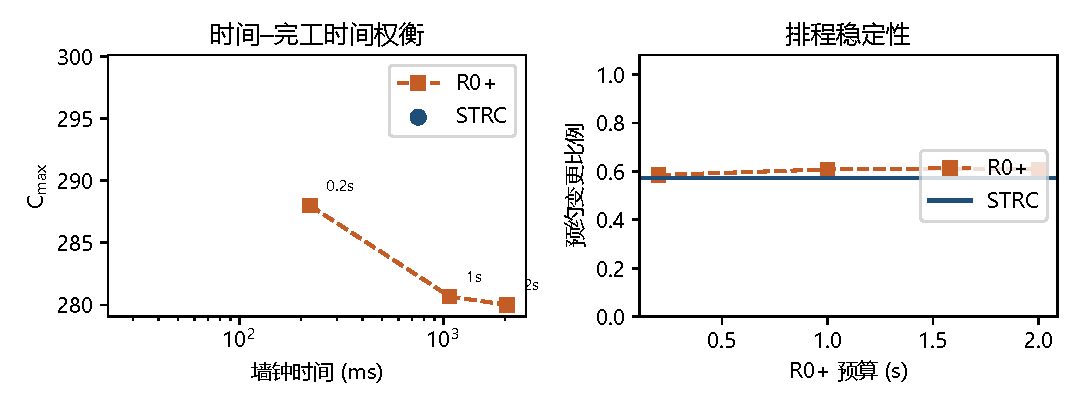
\includegraphics[width=\linewidth]{figures/fig_strc_e5_CN}
\caption{E5:不改写已结束占用的 R0+ 预算扫描与有界修复定点(\texttt{congested\_8x4x4}, \(3\) 个随机种子均值)。
左:算法耗时--\(C_{\max}\),两条曲线不相交;右:占用改动比例,两法同在六成附近。}
\Description{并排两幅图。左幅横轴为对数刻度的算法耗时、纵轴为完工时间:
不改写已结束占用的热启动全局重调度随预算略降,有界修复是左上方的一个定点,
两者不相交,全局重调度在每个预算点上都略低。右幅为占用改动比例,
两法都在六成附近,不再是百分之百对六成。}
\label{fig:e5}
\end{figure}

有界修复的完工时间全区间较差;算法耗时低两至三个数量级(以第 1 级改路的 \(\MsRepairMed\)\,ms
对 \(0.2\)--\(2\)\,s 预算计,见图~\ref{fig:e5} 左)。这一耗时差来自单遍改路、不重开搜索,
\emph{不是}影响集划界的功劳——第~\ref{sec:cheap}~节以耗时相同的 RA 对照坐实这一点。
与 R0+ 的改动比例则已同在 \ResFracRtwo\ 量级
(少改写须看第~\ref{sec:cheap}~节与 RA 的对照:两边改写比例已经接近,不能从本表读出稳定性)。
响应须在毫秒量级时,有界修复能恢复可行;允许秒级停机时,不改写已结束占用的热启动全局重调度在完工时间上仍占优,
但优势幅度已远小于从 \(t=0\) 重排的那一档。
\(C_{\max}\) 是本领域的主指标,故按它报告。
第~\ref{sec:vs_r0}~节所说的对照,指的是两者在\emph{算法耗时}约束下各自可用,不是指存在某个预算区间使 R2 的 \(C_{\max}\) 更优。

本表的 R0+ 按第~\ref{sec:vs_r0}~节的固定前缀解码,不改写已经结束的占用。
已结束占用不可改写的审计上,小例与拥堵例各 \(9\) 个预算点越界均为 \(\RzeroPastLo\);
同工件后道已出车、前道还要重定时,改为强制原车、只重规划 \(t_{\mathrm{now}}\) 之后的尾段,
历史空载前缀得以保留。有界修复在同样这些格上仍一律为零。
与「从 \(t=0\) 重排」的旧对照相比,\(C_{\max}\) 差距大幅收窄,改动比例不再是
百分之百对六成;但两者的次序未变,仍无交叉。缺口里原先混着的「改写已经结束的占用」已经被拿掉,
剩下的是全局改派改序相对单遍改路的那一截。
就贡献而言,本节只落一条\emph{限定}:预约影响集的净作用不在完工时间上,适用位置是毫秒档;
净作用究竟是什么,由第~\ref{sec:cheap}~节的 RA 对照回答。

\subsection{E7:毫秒档内的对照}
\label{sec:cheap}

上一节的对照是热启动种群搜索,预算 \(0.2\)--\(2\)\,s。只用它作对照会留下一个问题:
\emph{「低两至三个数量级」这个读数,有多少来自预约影响集,又有多少只是因为对照耗时更长?}
本节把阶梯中间那两档耗时更短的全局重算补上。

\begin{itemize}[leftmargin=1.5em,itemsep=0.25em]
\item \textbf{RS(全局右移)。} 不改路径、不改指派、不改扫描序,把未完成占用整体后推
一个延迟 \(\Delta\),\(\Delta\) 取到刚好让受阻走廊上所有可动的占用落到阻断窗之后。
不改写已经结束的占用(\(t_{\mathrm{end}}\le t_{\mathrm{now}}\) 不可动),与 R2 相同;
因为是统一平移,一切间隔要么不变、要么变大,而全部约束都是「\(\ge\)」型,
无需重新路由即得可行解。它是「\emph{不按影响集划界}」的一端:连改路都放弃
(第~\ref{sec:rw_aor}~节)。
\item \textbf{RD(原染色体重解码)。} 保持机器指派与扫描序,在装了阻断的路由层上
走与 R0+ 同一套固定前缀解码。它是本文实现里\emph{耗时更短的一次全局重算};不改染色体,因而比 R0+ 耗时更短,
也更少改派改序的自由度。
\item \textbf{RA(不按影响集限制范围,但保留改路)。} 把 \(t_{\mathrm{now}}\) 之后\emph{尚未结束}的占用全部纳入改写,
再走与 R2 \emph{完全相同}的改路重放。它是「不按影响集划界」的另一端:与 RS 不同,它保留了
改路,因而与 R2 只差允许改写哪些占用。两者同一套改路程序,都不改已经结束的占用,共用同一段阻断。
因此它是本文\emph{唯一}能把预约影响集单独隔离出来的对照——两法之差不含改路程序、协议或实现的贡献。
RA 已是最大允许改写集合,无需失败后扩大范围。
\end{itemize}

E3 比较的是两种\emph{不同}的划界对象(工序依赖图 vs 预约影响集),而 RA 问的是:
\emph{要不要按影响集限制范围}。

\begin{table}[t]
\centering
\caption{E7 毫秒档内对照(\(\NPairs\) 对,协议与 E3 相同:繁忙走廊单窗阻断、
\(t_{\mathrm{now}}=0.35\,C_{\max}^{0}\)、R2 不扩大范围)。四法均 \(\NPairs/\NPairs\) 可行。
「已结束占用越界」为改写了已结束占用的格数;「允许改写」为该方法纳入改写的占用占 \(t_{\mathrm{now}}\)
之后尚未结束占用的比例;末列为该方法对 R2 的 \(C_{\max}\) 胜负。RA 与 R2 只差允许改写哪些占用,
故这两行之差可全部归因于预约影响集。本表\emph{不可}与表~\ref{tab:e5} 并读——那批只有两个算例。}
\label{tab:cheap}
\small
\begin{tabular}{@{}lcccccc@{}}
\toprule
方法 & 已结束占用越界 & ms(中位) & 平均退化 & 改动比例 & 允许改写 & 对 R2 赢/平/输 \\
\midrule
RS 全局右移      & \ShiftBad     & \MsShift    & \(58.8\%\) & \ResFracShift    & ---   & \(7/16/27\) \\
RD 重解码        & \RedecodeBad  & \MsRedecode & \(49.0\%\) & \ResFracRedecode & ---   & \(22/14/14\) \\
RA 不按影响集划界 & \ShiftBad     & \MsAllFuture & \(49.9\%\) & \ResFracAllFuture & \(1.00\) & \(0/46/4\) \\
R2 有界修复      & \ShiftBad     & \MsCheapRtwo & \(49.8\%\) & \ResFracCheapRtwo & \ClosureShareMean & --- \\
\bottomrule
\end{tabular}
\end{table}

表~\ref{tab:cheap} 给出四条读数。

\textbf{其一,在给出可行方案的各法中,唯一比有界修复更快的是全局右移,
而它在完工时间与改写比例上都较差。}(按工序依赖图划界的 R1 更快,但它在 \FeasRone\ 上恢复可行,
不构成候选。)
RS 只要 \MsShift\,ms,约为 R2 的一半;代价是完工时间平均退化 \(58.8\%\)(R2 为
\(49.8\%\)),逐格对比 \WinVsShift(R2 赢/平/输),且改动的占用反而更多
(\ResFracShift\ 对 \ResFracCheapRtwo)——统一平移把每一条尚未结束占用的时刻都改了。
若想把右移做得\emph{有选择}——只推迟真正受影响的车,其余不动——就必须先
知道哪些占用受影响,那正是本文划定的范围。\textbf{右移之所以能不按影响集划界,恰恰因为
它放弃了选择。}

\textbf{其二,耗时更短的一次全局重算仍比一次有界修复更长。} RD 的耗时中位数是
\MsRedecode\,ms,为 R2 的 \RedecodeRatio\ 倍。这条读数与搜索配置无关:任何基于解码的搜索,
每评估一个候选都要付至少一次解码的代价。因此上一节「低两至三个数量级」并\emph{不}是
对照选得耗时更长造成的——把对照换成同一实现里耗时更短的那一档,有界修复仍然更快。

\textbf{其三,不改写已结束占用之后,RD 与 R2 的完工时间在本样本上不可区分,但 RD 改动更多。}
全表看 R2 对它是 \WinVsRedecode(赢/平/输),平均退化 \(49.8\%\) 对 \(49.0\%\)。这一差别经不起检验:
配对差均值 \(+0.006\),bootstrap \(95\%\) 区间 \([-0.007,\,0.019]\) 跨过 \(0\);Wilcoxon 符号秩
双侧 \(p=0.12\)(非零差 \(36\) 格);\(C_{\max}\) 比值均值 \(0.997\)、区间 \([0.988,\,1.007]\) 亦跨过 \(1\)。
故此处只报「未观察到差异」,不报方向。
已结束占用越界已是 \RedecodeBad:降级后道改为强制原车、只重规划决策时刻之后的尾段,
历史空载前缀不再丢。故即便逐格计数上 RD 略占上风,也不能把它写成「来自改写已经结束的占用」——这是同染色体、
只排未来时,全局改路相对单遍改路的那一截。改动比例 RD 为 \ResFracRedecode,高于 R2 的
\ResFracCheapRtwo:少改写仍在按影响集划界的一侧。

\textbf{其四,少改写只能从 R2 对 RA 读出,而且读到的只是稳定性。} RA 与 R2 只差允许改写哪些占用,因此这一对
读数直接回答了「按影响集划界值不值」。预约影响集平均只比平凡上界少纳入 \(1-\ClosureShareMean\)
的尚未结束占用(逐格 \ClosureShareLo--\(1.00\),取到 \(1.00\) 的 \(6\) 个格上影响集\emph{就是}
全部尚未结束占用,两法恒等)。就是这不足一成的差别,把改动比例从 \ResFracAllFuture\ 降到
\ResFracCheapRtwo:平均降 \RAStabMean、中位降 \RAStabMed,逐格 \RAStabWTL(R2 更稳/持平/更差),
Wilcoxon 符号秩双侧 \(p=\RAStabP\)。须说明有效样本量:上述 \(6\) 个恒等格不是两法的比较,
剔除后为 \(44\) 格、逐格 \RAStabWTLNet、平均降 \RAStabMeanNet(Wilcoxon 的非零差格数两种算法
下都是 \(32\));剔除使降幅估计\emph{变大},故按 \NPairs\ 格报告是偏保守的一侧。方向高度一致,\emph{幅度不大}——唯一的反例格上 R2 反而多改 \(0.007\),一并记下。与此同时算法耗时几乎相同(\MsCheapRtwo\ 对 \MsAllFuture\,ms),
完工时间也几乎相同(比值均值 \RACmaxRatio,逐格 R2 赢/平/输 \WinVsAllFuture、从未更差,
最占优的一格为 \RACmaxLo)。

这三项合起来才是重点。\textbf{耗时相同,说明毫秒级响应来自单遍改路、不重开搜索,而不是来自预约影响集
(读数见本节表~\ref{tab:cheap};单遍改路本身已是既有做法,见表~\ref{tab:position})。
完工时间相同,说明影响集不是一种优化手段。改动比例显著更低,说明划界落实的恰是命题
\ref{prop:outside} 承诺的那个量:集外占用的走廊、时段与车辆不变。}影响集的作用在于\emph{标出哪些占用不必改}。幅度随影响集排除得多而变大,方向一致,
但排除集本身只能解释其中一部分——被禁止改写的占用即便全部计入,也不足以补足
\(\ResFracAllFuture-\ResFracCheapRtwo\) 的全部落差,余下部分来自释放集变小后改路结果本身的
差异,本文不再细分:
在影响集接近全部尚未结束占用的算例上(\texttt{congested\_8x4x4},允许改写占比 \(0.94\))
降幅只有 \(0.010\),而在排除得多的算例上(\texttt{S8x4x4\_mid},\(0.91\))降幅达 \(0.118\)。% selfcheck:allow-num 0.91 为该算例的允许改写占比,与 \ScaleCloAliveHi(E8 档均值上界)同值不同源
两个算例定不出比例关系,能说的只是方向;逐格分布见下。

把这一方向写成一条事后分档。图~\ref{fig:worth} 以允许改写占比
\(\mathrm{Cl}/|R^{\circ}|\) 为横轴、RA 相对 R2 的改动比例降幅为纵轴,画出 \(\NPairs\) 对。
在本样本上取 \(\mathrm{Cl}/|R^{\circ}|\ge\WorthThresh\):该线以上 \WorthHighN\ 格平均降幅
\WorthHighMean,以下 \WorthLowN\ 格平均降幅 \WorthLowMean;
占比升到 \(\WorthVanish\) 以上的各格降幅均已归零,但成因有两种:占比恰为 \(1.00\) 的 \(6\) 格
影响集就是全部尚未结束占用,两法\emph{恒等};其余各格占比尚不足 \(1.00\) 而降幅已为 \(0\),
属实测而非恒等。
这是一条事后分档,阈值在本表上选定,不作外推定理;它回答的是「何时按影响集划界还值」,
不是影响集规模的结构预测(后者仍未建立,第~\ref{sec:e4}~节)。

\begin{figure}[t]
\centering
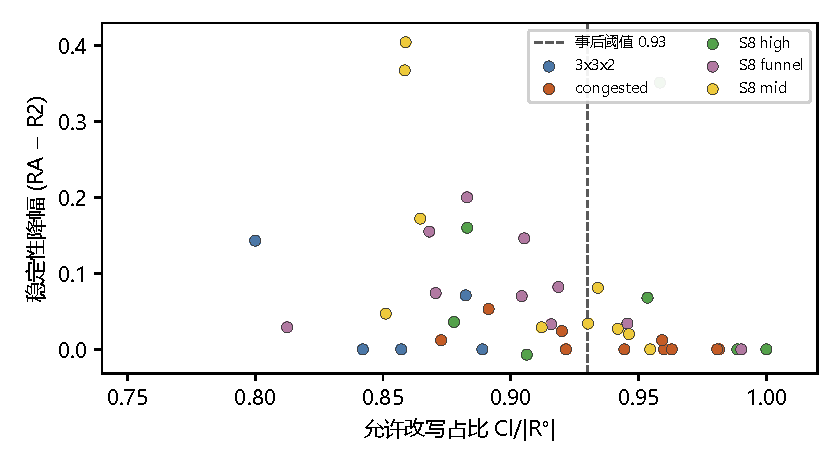
\includegraphics[width=0.92\linewidth]{figures/fig_strc_worth_CN}
\caption{E7 事后规则:允许改写占比与稳定性降幅(\(\NPairs\) 对,R2 对 RA)。
虚线为样本内阈值 \(\WorthThresh\);纵轴为正表示按影响集划界后改动比例更低。}
\Description{散点图,横轴为预约影响集占尚未结束占用的比例,纵轴为不按影响集划界相对划界多改的占用比例,
五个算例用不同颜色区分,一条竖虚线标在 \WorthThresh。点大致从左上到右下。}
\label{fig:worth}
\end{figure}

四法并读的收口是:在「不改写已经结束的占用、且响应在毫秒量级」这两个约束下,
\textbf{按影响集划界的净收益只体现在改写量上——同等速度、同等完工时间下,不划界要多改
约 \(6\) 个百分点的占用(相对多约一成二)},它\emph{不}包含速度或完工时间上的任何优势。
这一层回答的是「划界值不值」;「划界对象是否成立」由第~\ref{sec:e1}~至~\ref{sec:e3}~节支撑,
两层不可互相代入。放宽耗时约束后更短的完工时间仍来自热启动搜索(第~\ref{sec:e5}~节),
但那已不是毫秒档。

\subsection{扰动规模扫描}
\label{sec:scale}

表~\ref{tab:scale} 与图~\ref{fig:scale} 报告 \(\varphi\) 扫描
(\texttt{congested\_8x4x4}, \(\NSeeds\) 个随机种子; R0+ 预算 \(2\)\,s)。
逐档读数见表;\(C_{\max}\) 仍全由 R0+ 更优,与第~\ref{sec:e5}~节一致。
小例 \texttt{example\_3x3x2} 上同样每格可行(\(\NSeeds\) 个随机种子 \(\times\) 五个
\(\varphi\) 值),有界修复约 \(1\)\,ms 量级,
耗时比 \(\SpeedLo\times\)--\(\SpeedHi\times\)(跨两个算例的逐格极值)。这里分母是有界修复的
实测挂钟,分子是 R0+ 的\emph{预算},而 R0+ 在 \(C_{\max}\) 上更优,故它不是「加速比」,
也不构成同质量下的比较(第~\ref{sec:protocol}~节已声明各法不在同一预算档上比较)。

这里有界修复打开了失败后扩大范围,故与 E3/E5 不可直接比较:扩大范围是把可行率拉到 \(100\%\) 的
步骤,本身已有成例(第~\ref{sec:rw_aor}~节)。本节\emph{不支撑任何一条贡献},只落一条限定:
即使扰动比例升至 \(\varphi=1\)(全部未来工序受扰),算法耗时仍在十毫秒量级、不随规模崩溃;
这一耗时来自单遍改路,\emph{不是}影响集划界的功劳(第~\ref{sec:cheap}~节)。

\begin{table}[t]
\centering
\caption{扰动规模对照(\texttt{congested\_8x4x4}, \(\NSeeds\) 个随机种子平均)。
有界修复含扩大范围;R0+ 预算 \(2\)\,s。离散度按四分位距报告:STRC 耗时全扫描极差为
\ScaleMsMin--\ScaleMsMax\,ms,R0+ \(C_{\max}\) 的逐档 IQR 在 \ScaleCmaxIqrLo--\ScaleCmaxIqrHi
之间。\textbf{「耗时比」一列在最小两档上的档内 IQR 已超过该列的档间起落,
故它只作量级读数,不指示随 \(\varphi\) 的趋势。}该列为\emph{逐格}比值的档均值(先配对、后统计),
因此不等于相邻两列档均值之比——两者由 \(1/x\) 的凸性必然不同,复算时请用逐格数据。
分子是 R0+ 的挂钟\emph{预算}而非其实测耗时,故这不是同质量下的比较(第~\ref{sec:protocol}~节)。}
\label{tab:scale}
\small
\begin{tabular}{@{}rcccc@{}}
\toprule
\(\varphi\) & STRC 可行 & STRC\,ms & R0+ \(C_{\max}\) & 耗时比 \\
\midrule
\(0.10\) & \(100\%\) & \(9.1\)  & \(103.5\) & \(406\times\) \\
\(0.25\) & \(100\%\) & \(11.1\) & \(107.0\) & \(325\times\) \\
\(0.50\) & \(100\%\) & \(8.6\)  & \(111.8\) & \(333\times\) \\
\(0.75\) & \(100\%\) & \(8.4\)  & \(125.8\) & \(254\times\) \\
\(1.00\) & \(100\%\) & \(10.7\) & \(148.1\) & \(203\times\) \\
\bottomrule
\end{tabular}
\end{table}

\begin{figure}[t]
\centering
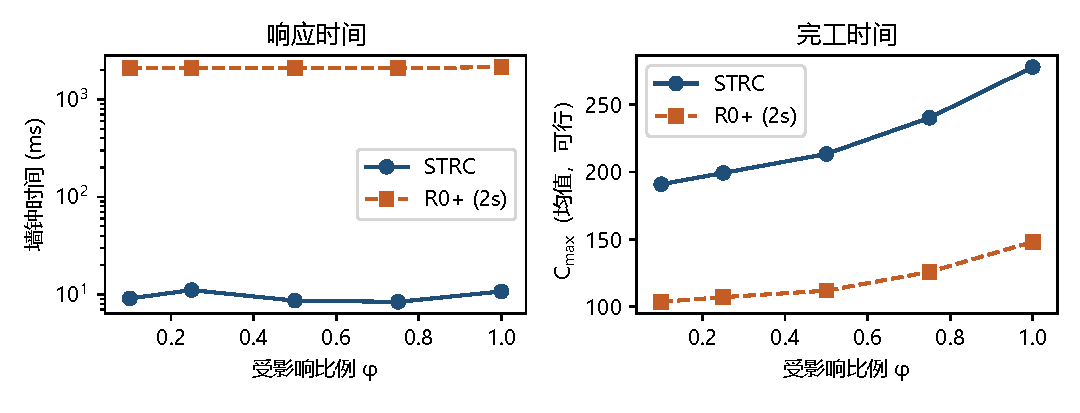
\includegraphics[width=\linewidth]{figures/fig_strc_scale_CN}
\caption{扰动规模扫描(\texttt{congested\_8x4x4}, \(\NSeeds\) 个随机种子):
有界修复与 R0+ 的算法耗时(对数轴)与完工时间随 \(\varphi\) 变化。曲线取逐档均值,
离散度口径与表~\ref{tab:scale} 同(四分位距);耗时一侧全扫描极差
\ScaleMsMin--\ScaleMsMax\,ms,始终在十毫秒量级,这是本节唯一据以立论的读数。}
\Description{两条随扰动比例变化的曲线。算法耗时画在对数纵轴上:有界修复始终在
十毫秒量级、不随比例上升而崩溃,全局重调度固定在两秒的预算线上。完工时间一侧,
全局重调度随扰动比例增大而缓慢上升,但始终低于有界修复。}
\label{fig:scale}
\end{figure}

\subsection{E8:算例规模上的外推}
\label{sec:instscale}

上一节扫的是\emph{扰动}的规模,算例始终是 \(8\) 工件 \(4\) 机。本节换一维:固定扰动协议,
把算例本身放大。这一问的要害不在耗时——耗时不崩是可以预期的——而在\textbf{影响集占比会不会
随规模涨到接近 \(1\),使「有界」名存实亡}。

梯子取工件数 \(2k\)、机器数 \(k\)、车数 \(k\),\(k=4,\dots,10\),即 \(8\times4\times4\) 到
\(\ScaleJobsHi\times\ScaleMachHi\times\ScaleMachHi\),共 \(\ScaleKs\) 档 \(\times\)
\(\NSeeds\) 个随机种子 \(=\ScalePairs\) 对。拥堵档、异构度、柔性度、运输/加工时长比与装卸点
最小割、远端割全部按同一目标标定,\emph{只有规模变}。三条对照与第~\ref{sec:cheap}~节同定义。

\begin{table}[t]
\centering
\caption{E8 算例规模扫描(\(\ScaleKs\) 档 \(\times\) \(\NSeeds\) 个随机种子)。
「影响集」为预约影响集占\emph{全表}之比,该比的可达上界是 \(|R^{\circ}|/|R|\)、本批均值约
\ScaleAliveShare;换以可改写集合为分母则为 \ScaleCloAliveLo--\ScaleCloAliveHi(见正文)。
耗时取中位数,「RD/R2」一列即两列\emph{中位数之比};正文讨论其单调性时用的是逐格配对后的
档均值,两种口径的档间起落一致但数值不同。末列为 R2 对 RS 的 \(C_{\max}\) 胜负。}
\label{tab:instscale}
\small
\begin{tabular}{@{}lrccccc@{}}
\toprule
规模 & \(|R|\) & 影响集 & R2\,ms & RD\,ms & RD/R2 & R2 对 RS \\
\midrule
\(8\times4\times4\)    & \(148\) & \(0.561\) & \(2.9\)  & \(4.4\)  & \(1.5\times\) & \(7/1/2\) \\
\(10\times5\times5\)   & \(172\) & \(0.485\) & \(3.2\)  & \(6.1\)  & \(1.9\times\) & \(9/0/1\) \\
\(12\times6\times6\)   & \(230\) & \(0.481\) & \(4.5\)  & \(10.7\) & \(2.4\times\) & \(7/1/2\) \\
\(14\times7\times7\)   & \(281\) & \(0.492\) & \(6.1\)  & \(14.5\) & \(2.4\times\) & \(8/0/2\) \\
\(16\times8\times8\)   & \(291\) & \(0.534\) & \(6.4\)  & \(16.4\) & \(2.6\times\) & \(10/0/0\) \\
\(18\times9\times9\)   & \(356\) & \(0.535\) & \(8.2\)  & \(26.4\) & \(3.2\times\) & \(10/0/0\) \\
\(20\times10\times10\) & \(402\) & \(0.476\) & \(10.4\) & \(34.2\) & \(3.3\times\) & \(10/0/0\) \\
\bottomrule
\end{tabular}
\end{table}

逐档读数见表~\ref{tab:instscale}。

\textbf{影响集占比不随规模恶化,但「接近 \(1\)」之疑须换分母才算回答。}
七档 \(\mathrm{Cl}/|R|\) 在 \ScaleCloLo--\ScaleCloHi 之间波动、并不单调
(首档最高、末档最低,第五、六两档回到 \(0.53\) 以上)。这里必须把分母交代清楚,
否则会读出过强的结论:\(\mathrm{Cl}\) 只取 \(t_{\mathrm{now}}\) 之后尚未结束的占用,
而本批 \(|R^{\circ}|/|R|\) 均值仅 \ScaleAliveShare,故 \(\mathrm{Cl}/|R|\) 的可达上界本就不是
\(1\) 而是约 \ScaleAliveShare——用它回答上面那一问并不切题。换成可改写集合作分母,
七档 \(\mathrm{Cl}/|R^{\circ}|\) 落在 \ScaleCloAliveLo--\ScaleCloAliveHi(逐格最高取到 \(1.00\)),
与第~\ref{sec:e6}、\ref{sec:cheap}~两节主批次的 \ClosureAliveFrac\ 同量级。
所以本节支持的是\emph{占比不随规模恶化},\emph{不是}「有界」在绝对量上宽裕——
后者已由注~\ref{rem:minimality} 否认。这也不是一个渐近主张:
七档不足以拟合任何增长率,能说的只是在这段区间内它没有退化。

\textbf{算法耗时的增长快于占用总数的增长。} \(|R|\) 增至 \(2.7\) 倍时,R2 的耗时中位数从
\(2.9\) 增至 \ScaleMsHi\,ms、即 \(3.6\) 倍,仍在十毫秒量级;七档定不出指数,
故这里只报两端之比,不写成「线性」或「超线性」。第 1 级改路的可行格数为 \ScaleFeasFirst;
唯一失败的一格(\(10\times5\times5\),随机种子 \(42\))由失败后扩大范围在第 \(3\) 轮兜住,
总耗时 \(12.0\)\,ms、完工时间与首级尝试相同,故终可行为 \ScaleFeasAll。

\textbf{两个对照的差距随规模拉大。} 耗时更短的全局重算与有界修复的耗时比
从 \ScaleRatioLo\(\times\) 升到 \ScaleRatioHi\(\times\)——规模越大,重算一遍越不划算。
这里只报两端:逐档比值\emph{并不单调}(逐格配对后的档均值在 \(k=6\to 7\) 处回落)。
两端相差 \(1.8\),而任一档内的四分位距不超过 \(0.74\)、每档 \NSeeds\ 格档均值的抽样波动
远小于该跨度,故\emph{总体在升}不是噪声;但增长形状本文不报;
而对不按影响集划界的右移,R2 的 \(C_{\max}\) 胜负在最后三档均为 \(10/0/0\),前四档则在
\(7\)--\(9\) 胜之间没有单调变化;每档只有 \NSeeds\ 格,故这里只报末三档的全胜,不报趋势。

\textbf{口径限制。} 这条梯子只有一个拥堵档、一个算例随机种子(每档的算例本身由随机种子
\(42\) 生成),因而它检验的是\emph{规模}这一维,不能替代第~\ref{sec:protocol}~节主批次在
拥堵结构上的对照;第~\ref{sec:e6}、\ref{sec:scale}~两节的扫描也未在这批算例上重跑。
就贡献而言,本节只为 C2 的有界性补一条\emph{规模方向}的限定:占比在这七档上没有被稀释,
但这不涉及净收益,也不构成渐近结论。

\subsection{外部布局批次的复现}
\label{sec:pubrepro}

第~\ref{sec:protocol}~节第二批把布局出处换成外部来源后,\(\NPubPairs\) 个算例--随机种子对上
E1/E2/E3/E5 的读数与主批次\emph{逐项同向}:
工序依赖图给出空范围 \PubPassMiss(结构泄漏计 \(0\)),结构包含性 \PubPassClosed,
集外字段逐条不变 \PubPassInvar;边界消融下第 1 级改路的可行格数为 \PubFeasRone,
按预约影响集划界为 \PubFeasRtwo。E1 协议下的影响集占比逐布局中位落在
\PubEoneFracLo--\PubEoneFracHi;同口径的主批次读数是 \NPairs\ 对合池中位 \EoneFracMed
(\EoneCloLo--\EoneCloHi\ 是逐算例\emph{均值}的极差,口径不同,不宜与上句直接对读)。
外部批整体略低,但两者同处半数上下的量级,且该偏低与逐算例间差异同量级
(第~\ref{sec:e1}~节图注);本文未对它作归因。
与全局重调度的权衡亦无变化:\PubEfiveNoCross\ 个预算点上 R0+ 的 \(C_{\max}\) 更优,
余下 \(1\) 点两法持平(\texttt{LyuL6\_8m},随机种子 \(2024\),预算 \(0.2\)\,s),无一点更差。
这批与主批次跑的是同一份 E5 代码、同一组参数,故第~\ref{sec:e5}~节按 \(\EfiveCells\) 个
算例--随机种子格合读两批;持平的那一格也满足该节的单调性判断,交叉点仍不存在。

这一批的意义不在于给出新的性能数字,而在于回答"这些现象是否只在本文自己设计的
布局上成立":上列三条读数在一批不由本文选定的拓扑上同样成立,故 C1 与 C2 的对象层
不依赖本文的布局设计。唯一被这批算例改写的结论是
结构可预测性(第~\ref{sec:e4}~节),而它本来就是负结果。

\subsection{小结}
\label{sec:exp_summary}

\begin{itemize}[leftmargin=1.5em,itemsep=0.25em]
\item E1 与边界消融(E3)在 \(\NPairs\) 个算例--随机种子对上无一例外成立;
案例甘特把同一协议落到工序时间轴。
\item 划界覆盖矩阵(E6)在四类扰动 \(\times\) \(\NPairs\) 对上给出划界读数:
A/B 二分无例外,且 A 类上预约影响集一致包含工序依赖图划界;修复一侧四类都开口:
B 类第 1 级均满(\FeasESixBlock / \FeasSlow),车辆故障换车 \FeasESixAgv,
机械臂故障改派 \FeasESixRa。
\item 结构包含性(E2a)与集外字段\emph{逐条}不变(E2b)均满通过;但这只说明
命题~\ref{prop:outside} 的四条前提在本文协议下成立,命题仍只作充分条件
(注~\ref{rem:e2b_history} 记录了前提 (iii) 曾如何在实现上被破坏)。
\item 与全局重调度相比,有界修复的 \(C_{\max}\) 在全部预算点上较差;两批合读的
\(\EfiveCells\) 个算例--随机种子格上,所测的 \(0.2\)--\(2\)\,s 区间内不存在交叉点,
且因 R2 为定点、R0+ 单调不增而可向更大预算外推;更小的预算未扫,那一侧不作断言。
算例维的普遍性则只到这些格子。算法耗时为毫秒对秒,
改动比例已与不改写已结束占用的 R0+ 同在 \ResFracRtwo\ 量级。
\item 毫秒档内对照(E7)排除了「对照耗时更长」这一疑问:在给出可行方案的各法中,唯一比有界
修复更快的是不按影响集划界的全局右移,而它在 \(C_{\max}\)(逐格 \WinVsShift)与改写比例
(\ResFracShift\ 对 \ResFracCheapRtwo)上都较差;同一实现里耗时更短的一次全局重算(原染色体
重解码)则比一次有界修复还长 \RedecodeRatio\ 倍。
\item 同一批还把预约影响集单独隔离出来测了一次:换用「不按影响集限制范围」的对照(RA,与 R2
同一套改路、都不改已经结束的占用),算法耗时与 \(C_{\max}\) 几乎不变,改动比例却由
\ResFracCheapRtwo\ 升到 \ResFracAllFuture(逐格 \RAStabWTL,\(p=\RAStabP\))。故毫秒级响应
来自单遍改路而非影响集;\textbf{少改写只能从这一对照读出},降幅随影响集排除得多而变大
(方向一致,不构成比例关系),样本内事后分档见图~\ref{fig:worth}。
\item 算例规模扫描(E8)把梯子推到 \(\ScaleJobsHi\) 工件 \(\ScaleMachHi\) 机:影响集占全表之比
在 \ScaleCloLo--\ScaleCloHi 间波动而不单调(该比的可达上界约 \ScaleAliveShare;
以可改写集合为分母则为 \ScaleCloAliveLo--\ScaleCloAliveHi,即有界性未随规模恶化,
但绝对量并不宽裕),算法耗时增长快于占用总数
升至 \ScaleMsHi\,ms,与重解码的耗时比由 \ScaleRatioLo\(\times\) 升到 \ScaleRatioHi\(\times\)
(端点在升,但逐档\emph{并不单调},见第~\ref{sec:instscale}~节)。
这是一段区间内的读数,不是渐近主张。
\item 预约影响集覆盖约 \(\ClosureAliveFrac\) 的尚未结束占用,不作最小性声称。
让行边纳入接壤后,差分试探在 \(\NPairs\) 对上泄漏为 \ProbeLeaks(\ProbeLeakPairs);
这只关闭了已观测到的那条通道。
\item 结构可预测性(E4)是负结果,且换用外部来源布局后更清楚:在\emph{同一张} \(4\times 4\)
外部路网上把机器配置由 \(4\) 机换成 \(5\) 机,影响集占比即变动 \PubCloSpread(该组仅 \(2\) 行;
\(5\times 5\) 那张上换三种配置为 \PubCloSpreadBig,自建路网间极差为 \SelfCloSpread\;
两侧变动的因子数不同,故这只支持「机器配置这一维不可忽略」),而 LU 最小割与漏斗占比
在整批外部算例上\emph{取值恒定},无从解释这一变动。替代方向指向需求侧的时序密度。
\item 两批算例承担不同的问题:主批次给出现象与机制,第二批只检验这些现象是否依赖本文
自选的布局。E1/E2/E3/E5 的读数逐项复现(\(\NPubPairs\) 对,第~\ref{sec:pubrepro}~节),
唯一被第二批改写的是结构可预测性——它也是唯一必须两批合读的一格
(第~\ref{sec:protocol}~节)。
\end{itemize}

以上按两层归并:\textbf{对象层}(C1、C2)由 E1、E2、E3、E6 与三条命题支撑;\textbf{净收益层}
(C3)只由 E7 的 RA 对照支撑——收益是少改写,\emph{不}含更快或更短的完工时间,速度来自单遍
改路而与划界无关。两层不可互相代入;E8 只为对象层补规模方向的限定,E4 是负结果、
不支撑任何贡献。


%% =====================================================================
\section{总结}
\label{sec:conclusion}
%% =====================================================================

本文有三项贡献。\textbf{其一},指认了一类工序依赖图覆盖不到的损坏:走廊阻断不改任何工序指派,
按受影响工序划出的范围为空而原排程确已不可行(\(\NPairs\) 对上 \(\PassMiss\),第~\ref{sec:e1}~节)。
\textbf{其二},把重调度范围定义为预约影响集(\STRC):依赖关系一经给定,一条占用是否属于该集
唯一确定,集内没有指向集外的依赖边(\(\PassClosed\)、\(\PassInvar\),第~\ref{sec:e2}~节);
这一层不依赖下面的净收益读数。
\textbf{其三},给出与该划界匹配的局部恢复,并分清各项读数各来自何处:同一套改路程序只换划界对象,
恢复可行率即由 \(\FeasRone\) 变到 \(\FeasRtwo\)(第~\ref{sec:e3}~节),
可行与否因此来自划界对象,而不是改路程序的优劣。

构成影响集的那几个机制——让行关系、集内改路而集外保持原计划、失败后扩大允许改写的范围——
分别已见于既有文献(第~\ref{sec:rw_claim}~节),本文不把它们当作贡献。本文主张的是:
工序依赖图按定义不含走廊占用之间的让行关系,因而覆盖不到只使占用失效的扰动;
改到预约依赖图上之后,须改写的占用由既定先后唯一确定,而不是一个启发式半径。

把允许改写的集合从预约影响集换成「\(t_{\mathrm{now}}\) 之后尚未结束的全部占用」、
其余一切不变时,算法耗时与完工时间几乎不动,改动比例却由 \ResFracCheapRtwo\ 升到
\ResFracAllFuture(第~\ref{sec:cheap}~节)。
故毫秒级响应来自单遍改路、不重开搜索;\textbf{少改写只能从这一对照读出,
落实的是命题~\ref{prop:outside} 承诺的量:集外占用保持原计划}。
收益幅度取决于影响集比平凡上界少纳入多少,因而在两者接近时趋于消失。

\subsection{局限}
\label{sec:limitations}

以下四条按对前文读数的影响排序,第~\ref{sec:future}~节逐条给出推进方向。

\begin{enumerate}[leftmargin=1.6em,itemsep=0.35em]
\item \textbf{完工时间上劣于不改写已结束占用的热启动全局重调度,
且在 \(\EfiveCells\) 个算例--随机种子格上放宽预算也不出现反超。}
对照已走固定前缀解码,已结束占用不可改写的审计为 \(\RzeroPastLo\)(第~\ref{sec:e5}~节),
E7 上 RD 越界同样为 \RedecodeBad。差距比从 \(t=0\) 重排时小得多,但方向没变:
有界修复换来的是算法耗时,交出的是完工时间。这\textbf{威胁}「划界值不值」这一层,
\textbf{不威胁}「改哪些占用由结构唯一确定」这一层——少改写只能从与 RA 的对照读出,
不能从对 R0+ 读出(第~\ref{sec:cheap}~节)。

\item \textbf{对预约影响集,保证仍只是充分条件,边集未经独立穷尽检验,
允许改写的集合不紧,规模也不可由只看路网的指标预测。}
四者分述;\textbf{威胁}的是对象层保证的强度与紧度,
\textbf{不威胁}「按工序划界会给出空范围」这一诊断读数。

\emph{(i) 命题~\ref{prop:outside} 只是充分条件},\(\PassInvar\) 不等于充要:
实验说明的是四条前提在本文协议下成立,不是它们可以省略。前提 (iii) 尤其脆弱——
只要实现以比占用更粗的粒度决定改路范围,\(U\) 外的占用就会被顺带改写
(注~\ref{rem:e2b_history})。逐条比对集外字段(E2b)兜不住这类错配,
本文对它的检出依赖于「事后想到该查什么」,而非一个完备的检查。

\emph{(ii) 依赖边集并不穷尽物理耦合,但已观测到的那条接壤通道已经关掉}。
差分试探——只把影响集内一条占用后移一个单位,观察集外是否出现新的同走廊重叠——
在把接壤并入让行边并重跑主矩阵之后, \(\NPairs\) 对上泄漏为 \ProbeLeaks
(\ProbeLeakPairs),同车方向始终为 \(0\)。这不是完备性证明:试探只覆盖「延后 \(1\)
个时间单位」这一种扰动(注~\ref{rem:minimality})。

\emph{(iii) 预约影响集不作最小性声称,且规模并不小}:它覆盖 \(t_{\mathrm{now}}\) 之后尚未结束占用的约
\(\ClosureAliveFrac\)(注~\ref{rem:minimality});相对「把尚未结束的占用全部纳入改写」这一平凡上界,
少纳入的不足一成。那不足一成的差别把改动比例降了 \RAStabMean
(逐格 \RAStabWTL,\(p=\RAStabP\);第~\ref{sec:cheap}~节的 RA),而算法耗时与 \(C_{\max}\) 不变:
限制不在于「划界无用」,而在于\textbf{收益幅度不大,且取决于影响集比平凡上界少纳入多少}——
在影响集接近全部尚未结束占用的算例上降幅仅 \(0.010\)。
把「何时值得」落成分档的规则(图~\ref{fig:worth})是样本内事后规则,不是结构预测,不能外推。

\emph{(iv) 影响集规模的结构可预测性未能建立,且已知不由静态割给出}:
装卸点最小割与漏斗占比都没有做出可复现的区分——这两个指标在整批外部算例上\emph{取值恒定}
(两张路网都把装卸站放在网格角点,四邻接下角点恰有两条出边),
而影响集占比在\emph{同一张}路网上单换机器配置就会变动:\(4\times 4\) 那张上由 \(4\) 机换
\(5\) 机即变动 \PubCloSpread,\(5\times 5\) 那张上换三种配置(\(6\)、\(7\)、\(8\) 机)变动
\PubCloSpreadBig(第~\ref{sec:e4}~节)。这条否定只针对「静态割能解释影响集规模」,
\emph{不是}「路网几何与影响集规模无关」——后者需要更多张互不相同的公开路网。

\item \textbf{实现覆盖仍窄于正文所述:修复一侧已满、恢复动作只有一档半、只做一次响应。}
\emph{扰动一维}四类均满,不构成限制
(\FeasESixBlock / \FeasSlow / \FeasESixAgv / \FeasESixRa,第~\ref{sec:e6}~节)。
\emph{动作一维},B 类仍只改路;A 类开口换车与改派,仍不改扫描序。
放开改序即向全局重调度退化,「有界」也随之失去边界。
\emph{时间一维},由假设 A3,扰动在 \(t_{\mathrm{now}}\) 完全已知且不叠加;
扰动流、预测误差与滚动响应均未涉及。
\emph{规模一维}的情况好一些但仍有限:第~\ref{sec:instscale}~节把梯子推到
\(\ScaleJobsHi\) 工件 \(\ScaleMachHi\) 机、\(\ScalePairs\) 对,影响集占比未随规模上升;
但那条梯子只有一个拥堵档与一个算例随机种子,\(\ScaleKs\) 档不足以支撑任何渐近论断。
本条\textbf{威胁}读数向更大规模与连续扰动的外推,\textbf{不威胁}协议内已报的读数。

\item \textbf{外部参照缺位:考虑执行期扰动的这一类研究没有可换的公开基准,算例出处只外部化了一半,
读数亦未在第二套实现上复现。}
公开算例族发布的都是静态问题的输入,
且把运输时间发布为机器间\textbf{行程时间矩阵}而不是路网——两族共 \(11\) 张布局逐张检验
\cite{homayouni2021production,bilge1995time},\emph{没有一张}能还原成与所发布矩阵一致的
无向走廊图;矩阵里没有走廊,\(R\)、\(G_R\)、\(\mathrm{Cl}(\cdot)\) 与 B 类扰动
在这类算例上\emph{一概无从定义}。
唯一发布显式双向排他路网的是 Lyu 等~\cite{lyu2019approach},本文已按其附录布局做出第二批
算例(第~\ref{sec:protocol}~节),\textbf{布局因此不再由本文设计};但外部化只做到拓扑一层
——\emph{逐段行驶时间与工件数据仍是本文的},这批算例因此\textbf{不能}用来复现
Lyu 或 van Os~\cite{vanos2026exact} 的参照值。
外部批次的\textbf{覆盖范围也窄于主批次}:它只复现 E1/E2/E3/E5(第~\ref{sec:pubrepro}~节),
且 \NPubInst\ 个算例只落在 \NPubNets\ 张路网上,路网几何这一维的样本量很小;
等权之外另扫的三档非均匀边权只重跑 E1/E3(R2 第 1 级可行率
\WeightLogRtwo、\WeightLuRtwo、\WeightSplitRtwo),替代不了一份同时发布路网与逐段时长的算例族。
最后,下层路网、时间窗路由与校验器\textbf{与静态一体化工作复用同一实现},
上述读数尚未在第二套独立实现上复现。
本条\textbf{威胁}外部效度,\textbf{不威胁}同一实现内各对照之间的相对读数。
\end{enumerate}

\subsection{后续工作}
\label{sec:future}

下列四条与上一节的四个局限一一对应。

\textbf{一、正视完工时间上的全区间劣势}(局限 \(1\))。
前缀解码对已结束占用的改写已在主批次收干净(E5 的 \(18\) 个预算点越界 \(\RzeroPastLo\),
E7 上 RD 为 \RedecodeBad)。局限 1 剩下的就是 \(C_{\max}\) 本身:不打算换加权指标绕过去。
若要缩小差距,需要的是在不改写已经结束占用的前提下做有限度改派或改序,那会向全局重调度退化。

\textbf{二、把预约影响集的保证做实、做紧,并给它的规模找一个刻画}(局限 \(2\))。
\emph{做实}:接壤已并入让行边,重跑后试探泄漏为 \ProbeLeaks。
下一步是换一种扰动形态(例如缩短占用、或延后超过 \(1\) 个单位)再探,而不是再补同一条边。
\emph{做紧},指向最小允许改写集合:在固定修复能力下定义最小性,
并给出影响集与之的差距,这是把「有界」从充分条件推进到紧界的必经一步;当前影响集覆盖约
\(\ClosureAliveFrac\) 的尚未结束占用,差距很可能不小。\emph{刻画规模}已有一条事后规则
(允许改写占比,图~\ref{fig:worth}),但它随排程而变;要换一族可在扰动前计算的指标:
第~\ref{sec:e4}~节已把静态割这一族排除——它在真实布局上取值恒定,而同一张路网上
单换机器配置就会变动:\(4\times 4\) 那张上由 \(4\) 机换 \(5\) 机即变动 \PubCloSpread,
\(5\times 5\) 那张上换三种配置(\(6\)、\(7\)、\(8\) 机)变动 \PubCloSpreadBig。
后者正好提示了方向:起作用的似乎是\emph{需求落在哪里}而不是路网提供了什么。
下一个候选是 \(t_{\mathrm{now}}\) 邻域内的走廊占用时序密度,例如受扰走廊在其繁忙窗口内的
重叠占用条数、以及该走廊在让行图上的出度。这类量随排程而变,不再是纯拓扑量,
「可预测性」的提法也须随之改为给定布局\emph{与当前排程}预测规模。

\textbf{三、放开假设 A3}(局限 \(3\);A3 为单次、完全观测)。
下一步不是再开改序,而是放开该条,考察影响集在连续扰动下是否会累积膨胀,
以及两次修复之间是否需要显式的「归位」步骤。

\textbf{四、把时间标定也外部化}(局限 \(4\))。布局出处已解决一半;要补齐另一半,
仍然需要一份同时发布\emph{排他路网与逐段时长}的算例族——自建边权扫不能替代它。
至于第二套独立实现,它不必单独立项——上述任何一件由他人复现时都会顺带完成。

%% 规范项收口:基金、致谢、利益冲突三项按期刊通例齐备。
%% acmart 的 acks 环境在 review/anonymous 模式下自动隐去,故匿名投稿无需手工删。
\begin{acks}
本文工作由 <待填:基金项目名称与编号> 资助。
作者感谢匿名审稿人对实验口径与结论边界提出的意见。
\end{acks}

\section*{利益冲突声明}
作者声明不存在与本文工作相关的利益冲突。

\bibliographystyle{ACM-Reference-Format}
\bibliography{reference-base}

\end{document}
